%!tex root=./thesis.tex

\appendix

\chapter*{Appendix}
\addcontentsline{toc}{chapter}{Appendix}
\markboth{Appendix}{}

\renewcommand{\thefigure}{\Alph{section}.\arabic{figure}}
\renewcommand{\thetable}{\Alph{section}.\arabic{table}}
\renewcommand{\theequation}{\Alph{section}.\arabic{equation}}
\numberwithin{figure}{section}
\numberwithin{table}{section}
\numberwithin{equation}{section}

\section{Classification models}\label{sec:atlas-xid-models}

  This appendix describes the three different models we used for binary classification in \autoref{cha:cross-id} (logistic
  regression, convolutional neural networks, and random forests) and was part of \citet{alger18radio}.

  \subsection{Logistic Regression}
  \label{sec:atlas-logistic-regression}
    Logistic regression is linear in the feature space and outputs the
    probability that the input has a positive label. The model is
    \citep{bishop06ml}:

    \begin{equation}
        f(\vec x) = \sigma(\vec w^T \vec x + b) \,\,\,\,,
    \end{equation}
    where $\vec w \in \mathbb{R}^D$ is a vector of parameters, $b \in \mathbb{R}$ is a bias term, $\vec x \in \mathbb{R}^D$ is the feature vector representation of a candidate host, and $\sigma : \mathbb{R} \to \mathbb{R}$ is the logistic sigmoid function: \begin{equation}
        \sigma(a) = (1 + \mathrm{exp}(-a))^{-1}\,\,\,\,.
    \end{equation}%
    The logistic regression model is fully differentiable, and the parameters
    $\vec w$ can therefore be learned using gradient-based optimisation
    methods. {We used the \texttt{scikit-learn} \citep{pedregosa11sklearn}
    implementation of logistic regression with balanced classes}.

  \subsection{Convolutional neural networks}
  \label{sec:atlas-convolutional-neural-networks}

    Convolutional neural networks (CNN) are a biologically-inspired prediction
    model for prediction with image inputs. The input image is convolved with
    a number of filters to produce output images called feature maps. These
    feature maps can then be convolved again with other filters on subsequent
    layers, producing a network of convolutions. The whole network is
    differentiable with respect to the values of the filters and the filters
    can be learned using gradient-based optimisation methods. The final layer
    of the network is logistic regression, with the convolved outputs as input
    features. For more detail, see \citet[subsection II.A][]{lecun98}. We used
    \textsc{Keras} \citep{chollet15keras} to implement our CNN, accounting for
    class imbalance by reweighting the classes.

    \begin{figure}
      \centering
      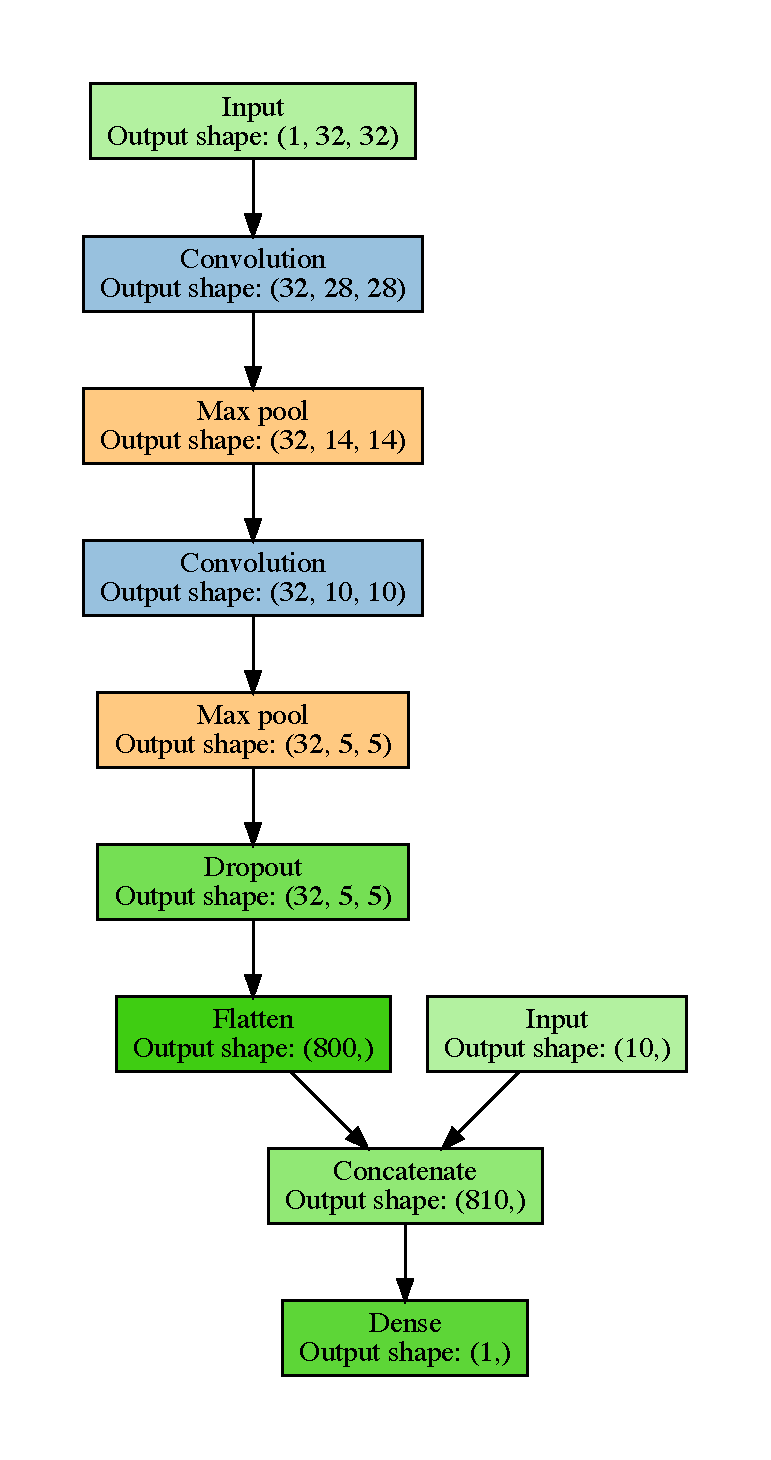
\includegraphics[height=0.9\textheight]{atlas-images/cnn_model_graph}
      \caption[Architecture of our CNN.]{Architecture of our CNN. {Parenthesised numbers indicate
      the size of output layers as a tuple (width, height, depth).} The
      concatenate layer flattens the output of the previous layer and adds the
      10 features derived from the candidate host in SWIRE, i.e. the flux
      ratios, stellarity indices, and distance. The dropout layer randomly
      sets $25\%$ of its inputs to zero during training to prevent
      overfitting. Diagram based on \url{ https://github.com/dnouri/nolearn}.}
      \label{fig:cnn}
    \end{figure}

    CNNs have recently produced good results on large image-based datasets in
    astronomy \citep[e.g.]{lukic18compact, dieleman15cnn}. We employed
    only a simple CNN model in \autoref{cha:cross-id} as a proof of concept that CNNs may
    be used for class probability prediction on radio images. The model
    architecture we used is shown in \autoref{fig:cnn}.

  \subsection{Random Forests}
  \label{sec:atlas-random-forests}

    Random forests are an ensemble of decision
    trees~\citep{breiman01random-forest}. They consider multiple subsamples of
    the training set, where each subsample is sampled with replacement from
    the training set. For each subsample a decision tree classifier is
    constructed by repeatedly making axis-parallel splits based on individual
    features. In a random forest the split decision is taken based on a random
    subset of features. To classify a new data point, the random forest takes
    the weighted average of all classifications produced by each decision
    tree. {In \autoref{cha:cross-id} we used the \texttt{scikit-learn} \citep{pedregosa11sklearn}
    implementation of random forests with 10 trees, the information entropy
    split criterion, a minimum leaf size of 45, and balanced classes}.

\section{Accuracy tables}\label{sec:atlas-xid-accuracies}
  
  This section contains tables of accuracy for our cross-identification method applied to CDFS and
  ELAIS-S1, and was originally presented in \citet{alger18radio}. In \autoref{tab:cdfs-ba} and \autoref{tab:elais-ba} we list the
  balanced accuracies of our \autoref{cha:cross-id} classifiers on the cross-identification task for CDFS
  and ELAIS-S1 respectively, averaged over each set of training quadrants. In
  \autoref{tab:cdfs-acc} and \autoref{tab:elais-acc} we list the balanced
  accuracies of classifiers on the cross-identification task for CDFS and
  ELAIS-S1 respectively, averaged over each set of training quadrants.

  \begin{table*}
    \caption[Balanced accuracies for different binary classification models on CDFS.]{Balanced accuracies for different binary classification models trained and tested on SWIRE objects in CDFS.
    The `Labeller' column states what set of training labels
    were used to train the classifier, and the `Classifier' column states what
    classification model was used. `CNN' is a convolutional neural network,
    `LR' is logistic regression and `RF' is random forests. Accuracies are evaluated against the expert
    label set derived from \citet{norris06}. The standard deviation of balanced accuracies evaluated across the four quadrants of
    CDFS (\autoref{fig:quadrants}) is also shown. The `compact' set refers to SWIRE
    objects within $1'$ of a compact radio component, the `resolved' set refers to
    SWIRE objects within $1'$ of a resolved radio component, and `all' is the union of these sets.}
    \label{tab:cdfs-ba}
    \small\centering
    \begingroup
    \setlength{\tabcolsep}{8pt} % Default value: 6pt
    \begin{tabular}{ccccc}
    \hline\hline
    Labeller & Classifier & Mean `Compact' & Mean `Resolved' & Mean `All'\\
     &  & accuracy & accuracy & accuracy\\
     &  & (per cent) & (per cent) & (per cent)\\
    \hline
    Norris & LR & $91.5 \pm 1.0$ & $93.2 \pm 1.0$ & $93.0 \pm 1.2$\\
     & CNN & $92.6 \pm 0.7$ & $91.2 \pm 0.5$ & $92.0 \pm 0.6$\\
     & RF & $96.7 \pm 1.5$ & $91.0 \pm 4.5$ & $96.0 \pm 2.5$\\
    RGZ & LR & $89.5 \pm 0.8$ & $90.5 \pm 1.7$ & $90.2 \pm 0.8$\\
     & CNN & $89.4 \pm 0.6$ & $89.6 \pm 1.3$ & $89.4 \pm 0.5$\\
     & RF & $94.5 \pm 0.2$ & $95.8 \pm 0.4$ & $94.7 \pm 0.3$\\
    \hline\hline
    \end{tabular}
    \endgroup
  \end{table*}

  \begin{table*}
    \caption[Balanced accuracies for different binary classification models on ELAIS-S1.]{Balanced accuracies for different binary classification models trained on SWIRE objects
    in CDFS and tested on SWIRE objects in ELAIS-S1. Columns and abbreviations are as in \autoref{tab:cdfs-ba}. Accuracies are evaluated against the expert
    label set derived from \citet{middelberg08}. The standard deviations of balanced accuracies of models trained on the four subsets of
    CDFS (\autoref{fig:quadrants}) are also shown.}
    \label{tab:elais-ba}
    \small\centering
    \begingroup
    \setlength{\tabcolsep}{8pt} % Default value: 6pt
    \begin{tabular}{ccccc}
      \hline\hline
      Labeller & Classifier & Mean `Compact' & Mean `Resolved' & Mean `All'\\
        &  & accuracy & accuracy & accuracy\\
        &  & (per cent) & (per cent) & (per cent)\\
      \hline
      Norris & LR & $94.6 \pm 0.4$ & $93.3 \pm 2.0$ & $95.3 \pm 0.1$\\
       & CNN & $94.8 \pm 0.2$ & $92.8 \pm 0.5$ & $94.4 \pm 0.2$\\
       & RF & $85.9 \pm 3.8$ & $70.0 \pm 2.8$ & $86.6 \pm 3.2$\\
      RGZ & LR & $91.8 \pm 0.3$ & $91.9 \pm 0.5$ & $92.0 \pm 0.2$\\
       & CNN & $90.1 \pm 0.3$ & $91.1 \pm 0.9$ & $90.2 \pm 0.3$\\
       & RF & $95.1 \pm 0.1$ & $95.2 \pm 0.0$ & $95.2 \pm 0.3$\\
      \hline\hline
    \end{tabular}
    \endgroup
  \end{table*}

  \begin{table*}
    \caption[Cross-identification accuracies for different classification
    models on CDFS.]{Cross-identification accuracies for different classification
    models on CDFS. The `Labeller' column states what set of training labels
    were used to train the method, and the `Classifier' column states what
    classification model was used. `CNN' is a convolutional neural network,
    `LR' is logistic regression, `RF' is random forests, and `Labels' is the
    accuracy of the label set itself. `Perfect' indicates that the true labels
    of the test set were used and hence represents an upper bound on
    cross-identification accuracy with our method. `NN' is a
    nearest neighbours approach. Accuracies are evaluated against the expert
    label set, so `Norris' labels are 100 per cent accurate by definition. The
    standard deviation of accuracies evaluated across the four quadrants of
    CDFS (\autoref{fig:quadrants}) is also shown.}
    \label{tab:cdfs-acc}
    \small\centering
    \begingroup
    \setlength{\tabcolsep}{8pt} % Default value: 6pt
    \begin{tabular}{ccccc}
      \hline\hline
      Labeller & Classifier & Mean `Compact' & Mean `Resolved' & Mean `All'\\
       &  & accuracy & accuracy & accuracy\\
       &  & (per cent) & (per cent) & (per cent)\\
      \hline
     ---& NN & $97.2 \pm 1.7$ & $75.7 \pm 7.9$ & $93.4 \pm 0.8$\\
     ---& Random & $97.9 \pm 2.2$ & $22.3 \pm 9.2$ & $83.2 \pm 4.7$\\
      Norris & Labels & $100.0 \pm 0.0$ & $100.0 \pm 0.0$ & $100.0 \pm 0.0$\\
             & Perfect & $97.9 \pm 2.2$ & $99.0 \pm 1.8$ & $98.1 \pm 1.7$\\
             & LR & $97.3 \pm 0.5$ & $76.0 \pm 3.2$ & $93.7 \pm 1.8$\\
             & CNN & $96.6 \pm 0.9$ & $74.3 \pm 12.3$ & $93.5 \pm 0.5$\\
             & RF & $96.1 \pm 1.4$ & $75.8 \pm 6.7$ & $93.8 \pm 2.0$\\
      RGZ & Labels & $53.1 \pm 8.5$ & $56.7 \pm 5.9$ & $54.4 \pm 5.9$\\
          & LR & $97.3 \pm 1.9$ & $74.5 \pm 5.1$ & $93.6 \pm 1.7$\\
          & CNN & $85.4 \pm 2.6$ & $68.1 \pm 9.2$ & $92.4 \pm 1.1$\\
          & RF & $97.5 \pm 0.9$ & $74.3 \pm 7.9$ & $93.7 \pm 1.5$\\
      \hline\hline
    \end{tabular}
    \endgroup
  \end{table*}

  \begin{table*}
    \caption[Cross-identification accuracies for different classification
    models on ELAIS-S1.]{Cross-identification accuracies for different classification
    models on ELAIS-S1. Columns and abbreviations are as in
    \autoref{tab:cdfs-acc}. Accuracies are evaluated against the expert label
    set derived from \citet{middelberg08} cross-identifications. The standard
    deviation of accuracies evaluated across models trained on the four
    quadrants of CDFS (\autoref{fig:quadrants}) is also shown.}
    \label{tab:elais-acc}
    \small\centering
    \begingroup
    \setlength{\tabcolsep}{8pt} % Default value: 6pt
    \begin{tabular}{ccccc}
      \hline\hline
      Labeller & Classifier & Mean `Compact' & Mean `Resolved' & Mean `All'\\
       &  & accuracy & accuracy & accuracy\\
       &  & (per cent) & (per cent) & (per cent)\\
      \hline
     ---& NN & $95.5 \pm 0.0$ & $92.8 \pm 0.0$ & $95.5 \pm 0.0$\\
     ---& Random & $61.9 \pm 1.1$ & $26.6 \pm 2.1$ & $61.9 \pm 1.1$\\
      Middelberg & Perfect & $99.6 \pm 0.0$ & $99.8 \pm 0.0$ & $99.6 \pm 0.0$\\
      Norris & LR & $89.0 \pm 1.1$ & $89.7 \pm 1.8$ & $94.4 \pm 0.9$\\
             & CNN & $89.7 \pm 0.3$ & $89.4 \pm 1.4$ & $94.3 \pm 0.7$\\
             & RF & $83.8 \pm 5.6$ & $82.3 \pm 4.1$ & $90.6 \pm 2.1$\\
      RGZ & LR & $90.5 \pm 1.0$ & $92.7 \pm 0.2$ & $95.9 \pm 0.1$\\
          & CNN & $84.6 \pm 0.6$ & $84.6 \pm 0.6$ & $91.8 \pm 0.3$\\
          & RF & $91.3 \pm 1.0$ & $90.3 \pm 2.4$ & $94.7 \pm 1.2$\\
      \hline\hline
    \end{tabular}
    \endgroup
  \end{table*}

\section{SWIRE object scores}\label{sec:atlas-xid-scores}
  
  This appendix is from \citet{alger18radio}, and contains scores predicted by our \autoref{cha:cross-id} binary classifiers for each
  SWIRE object within $1'$ of a radio component in CDFS and ELAIS-S1. Scores
  for SWIRE~CDFS objects are shown in \autoref{tab:cdfs-scores} and scores for
  SWIRE~ELAIS-S1 are shown in \autoref{tab:elais-scores}. For CDFS, the score
  for an object in a quadrant is predicted by binary classifiers trained on
  all other quadrants. For ELAIS-S1, we show the scores predicted by binary
  classifiers trained on each CDFS quadrant. Note that these scores have
  \emph{not} been weighted by Gaussians. These are partial tables, and the full tables are available online at the \emph{Monthly Notices of the Royal Astronomical Society} website\footnote{\url{https://doi.org/10.1093/mnras/sty1308}}.

  The columns of the score tables are defined as follows:
  \begin{itemize}
    \item \emph{SWIRE}---SWIRE designation for candidate host galaxy.
    \item \emph{RA}---Right ascension (J2000).
    \item \emph{Dec}---Declination (J2000).
    \item \emph{Expert host}---Whether the candidate host galaxy is a host galaxy according to \citet{norris06} or \citet{middelberg08} cross-identifications of CDFS and ELAIS-S1 respectively.
    \item \emph{RGZ host}---Whether the candidate host galaxy is a host galaxy according to Radio Galaxy Zoo cross-identifications \citep{wong21rgz}. This is always `no' for ELAIS-S1 objects.
    \item \emph{$C$/$L$/$D$}---Score assigned by binary classifier $C$ trained on label set $L$ of $D$ candidate host galaxies. $C$ may be `CNN', `LR' or `RF' for CNN, logistic regression or random forests respectively. $L$ may be `Norris' or `RGZ' for expert and Radio Galaxy Zoo labels respectively. $D$ may be `All', `Compact' or `Resolved' for each respective subset defined in \autoref{sec:atlas-xid-experimental-setup}.
  \end{itemize}

  \begin{sidewaystable}
    \caption[Scores output by our trained classifiers for SWIRE~CDFS candidate host galaxies.]{Scores output by our trained classifiers for SWIRE~CDFS candidate host galaxies. Columns are defined in \autoref{sec:atlas-xid-scores}. Full table electronic.}
    \label{tab:cdfs-scores}
    \small\centering
    \begin{tabular}{ccccccccccc}
      \hline\hline
SWIRE & RA & Dec & Expert & RGZ & \multicolumn{6}{c}{CNN}\\
& & & host & host & \multicolumn{3}{c}{Norris} & \multicolumn{3}{c}{RGZ}\\
& & & & & All & Compact & Resolved & All & Compact & Resolved\\
      \hline
J032603.15-284708.5 & 51.5132 & -28.7857 & yes & no & 0.5838 & 0.4697 & 0.4848 & 0.3754 & 0.3881 & 0.3404 \\
J032603.39-284010.1 & 51.5142 & -28.6695 & no & no & 0.0373 & 0.5814 & 0.4878 & 0.7896 & 0.7616 & 0.4668 \\
J032603.44-284210.1 & 51.5144 & -28.7028 & no & no & 0.0232 & 0.4891 & 0.5101 & 0.4319 & 0.4298 & 0.3474 \\
J032603.44-284222.2 & 51.5143 & -28.7062 & no & no & 0.0006 & 0.4164 & 0.5216 & 0.0400 & 0.0444 & 0.0276 \\
J032603.45-284748.4 & 51.5144 & -28.7968 & no & no & 0.0014 & 0.4914 & 0.4865 & 0.1904 & 0.1895 & 0.1467 \\
J032603.50-284637.0 & 51.5146 & -28.7770 & no & no & 0.0074 & 0.4144 & 0.5382 & 0.1418 & 0.1515 & 0.1166 \\
J032603.60-284627.4 & 51.5150 & -28.7743 & no & no & 0.0012 & 0.4578 & 0.5165 & 0.0850 & 0.0904 & 0.0484 \\
J032603.63-283840.5 & 51.5151 & -28.6446 & no & no & 0.0021 & 0.4153 & 0.5577 & 0.1678 & 0.1746 & 0.1323 \\
J032603.66-283822.8 & 51.5153 & -28.6397 & no & no & 0.0001 & 0.4752 & 0.5009 & 0.0864 & 0.0861 & 0.0613 \\
J032603.75-284014.1 & 51.5156 & -28.6706 & no & no & 0.0547 & 0.3408 & 0.5388 & 0.4889 & 0.5242 & 0.7301 \\
      \hline\hline
    \end{tabular}\\
    \begin{tabular}{cccccccccccc}
      \hline\hline
\multicolumn{6}{c}{LR} & \multicolumn{6}{c}{RF} \\
\multicolumn{3}{c}{Norris} & \multicolumn{3}{c}{RGZ} & \multicolumn{3}{c}{Norris} & \multicolumn{3}{c}{RGZ} \\
All & Compact & Resolved & All & Compact & Resolved & All & Compact & Resolved & All & Compact & Resolved \\
      \hline
0.2489 & 0.0009 & 0.1557 & 0.2939 & 0.0007 & 0.1174 & 0.8922 & 0.8018 & 0.8732 & 0.7167 & 0.6599 & 0.7801 \\
0.0183 & 0.1646 & 0.1480 & 0.7637 & 0.7065 & 0.6070 & 0.0000 & 0.0000 & 0.0000 & 0.1629 & 0.0519 & 0.1275 \\
0.0155 & 0.0164 & 0.0815 & 0.3714 & 0.5626 & 0.2488 & 0.0000 & 0.0734 & 0.0000 & 0.1315 & 0.2116 & 0.4150 \\
0.0005 & 0.0006 & 0.0175 & 0.0460 & 0.0810 & 0.0299 & 0.2656 & 0.1418 & 0.0000 & 0.7631 & 0.8166 & 0.5378 \\
0.0013 & 0.0037 & 0.0160 & 0.1792 & 0.0663 & 0.1821 & 0.0000 & 0.0000 & 0.0000 & 0.0255 & 0.0000 & 0.0000 \\
0.0047 & 0.0010 & 0.0337 & 0.1284 & 0.2198 & 0.0694 & 0.0720 & 0.0000 & 0.0000 & 0.6240 & 0.6681 & 0.6704 \\
0.0008 & 0.0006 & 0.0374 & 0.1053 & 0.1424 & 0.0807 & 0.1231 & 0.0876 & 0.0000 & 0.8517 & 0.7532 & 0.7019 \\
0.0021 & 0.0073 & 0.0386 & 0.1482 & 0.0403 & 0.1210 & 0.0000 & 0.0532 & 0.0000 & 0.0000 & 0.0302 & 0.0000 \\
0.0001 & 0.0004 & 0.0038 & 0.0854 & 0.0447 & 0.0514 & 0.0000 & 0.0000 & 0.0000 & 0.0000 & 0.0000 & 0.0000 \\
0.0542 & 0.2712 & 0.2318 & 0.5026 & 0.5631 & 0.5032 & 0.0595 & 0.0545 & 0.0000 & 0.4289 & 0.0789 & 0.1420 \\
      \hline\hline
    \end{tabular}
  \end{sidewaystable}

  \begin{sidewaystable}
    \caption[Scores output by our trained classifiers for SWIRE~ELAIS-S1 candidate host galaxies.]{Scores output by our trained classifiers for SWIRE~ELAIS-S1 candidate host galaxies. Columns are defined in \autoref{sec:atlas-xid-scores}. Full table electronic.}
    \label{tab:elais-scores}
    \small\centering
    \begin{tabular}{ccccccccccc}
      \hline\hline
SWIRE & RA & Dec & Expert & RGZ & \multicolumn{6}{c}{CNN} \\
 & & & host & host & \multicolumn{3}{c}{Norris} & \multicolumn{3}{c}{RGZ} \\
 & & & & & All & Compact & Resolved & All & Compact & Resolved \\
      \hline
J002925.73-440256.2 & 7.3572 & -44.0490 & yes & no & 0.9537 & 0.8638 & 0.5552 & 0.9195 & 0.9037 & 0.9371\\
J002926.14-440249.0 & 7.3590 & -44.0470 & no & no & 0.7361 & 0.8752 & 0.5640 & 0.7740 & 0.7474 & 0.7952\\
J002926.52-440247.0 & 7.3605 & -44.0464 & no & no & 0.3390 & 0.8338 & 0.5556 & 0.7275 & 0.6894 & 0.7197\\
J002926.63-440301.1 & 7.3610 & -44.0503 & no & no & 0.2108 & 0.8251 & 0.5623 & 0.3434 & 0.3306 & 0.3292\\
J002927.13-440232.6 & 7.3631 & -44.0424 & no & no & 0.0339 & 0.8479 & 0.5669 & 0.5853 & 0.5148 & 0.5159\\
J002927.28-440245.3 & 7.3637 & -44.0459 & no & no & 0.0406 & 0.8345 & 0.5540 & 0.2702 & 0.2340 & 0.2133\\
J002927.44-440238.5 & 7.3644 & -44.0440 & no & no & 0.0116 & 0.8267 & 0.5746 & 0.2228 & 0.2182 & 0.2028\\
J002928.08-440230.3 & 7.3670 & -44.0418 & no & no & 0.0024 & 0.8626 & 0.5791 & 0.2297 & 0.1963 & 0.1549\\
J002928.11-440312.7 & 7.3671 & -44.0535 & no & no & 0.0011 & 0.8159 & 0.5514 & 0.0377 & 0.0384 & 0.0271\\
J002928.80-440306.8 & 7.3700 & -44.0519 & no & no & 0.0003 & 0.8405 & 0.5668 & 0.0236 & 0.0226 & 0.0136\\
      \hline\hline
    \end{tabular}\\
    \begin{tabular}{cccccccccccc}
      \hline\hline
\multicolumn{6}{c}{LR} & \multicolumn{6}{c}{RF} \\
\multicolumn{3}{c}{LR} & \multicolumn{3}{c}{LR} & \multicolumn{3}{c}{RF} & \multicolumn{3}{c}{RF} \\
All & Compact & Resolved & All & Compact & Resolved & All & Compact & Resolved & All & Compact & Resolved \\
      \hline
0.9722 & 0.9955 & 0.8769 & 0.9933 & 0.9934 & 0.9658 & 0.8824 & 0.9664 & 0.7950 & 0.8078 & 0.9227 & 0.7677 \\
0.4669 & 0.0111 & 0.4249 & 0.3926 & 0.2220 & 0.5947 & 0.2077 & 0.0000 & 0.1613 & 0.1876 & 0.0852 & 0.4546 \\
0.2264 & 0.0254 & 0.2389 & 0.6275 & 0.3033 & 0.6812 & 0.1347 & 0.0857 & 0.0399 & 0.3582 & 0.4854 & 0.5347 \\
0.0603 & 0.0007 & 0.0734 & 0.0688 & 0.0141 & 0.1581 & 0.0917 & 0.0000 & 0.0399 & 0.2846 & 0.1245 & 0.2833 \\
0.0248 & 0.0334 & 0.0301 & 0.5735 & 0.5065 & 0.5265 & 0.1977 & 0.1507 & 0.0000 & 0.3334 & 0.6593 & 0.3995 \\
0.0173 & 0.0016 & 0.0359 & 0.1056 & 0.0492 & 0.1456 & 0.0000 & 0.0000 & 0.0000 & 0.0000 & 0.0000 & 0.0287 \\
0.0064 & 0.0049 & 0.0187 & 0.1981 & 0.1534 & 0.1493 & 0.0000 & 0.0000 & 0.0000 & 0.1565 & 0.1634 & 0.1284 \\
0.0020 & 0.0005 & 0.0239 & 0.1337 & 0.1001 & 0.1310 & 0.0000 & 0.0000 & 0.0358 & 0.0000 & 0.0000 & 0.0190 \\
0.0008 & 0.0013 & 0.0119 & 0.0280 & 0.0361 & 0.0205 & 0.1171 & 0.0000 & 0.0000 & 0.0873 & 0.0383 & 0.0000 \\
0.0004 & 0.0014 & 0.0095 & 0.0339 & 0.0408 & 0.0136 & 0.0000 & 0.0000 & 0.0000 & 0.1114 & 0.1480 & 0.1584 \\
      \hline\hline
    \end{tabular}
  \end{sidewaystable}

\section{ATLAS component cross-identifications}\label{sec:atlas-xid-xids}
  
  This section contains cross-identifications predicted by our \autoref{cha:cross-id} cross-identification method for each
  ATLAS radio component in CDFS and ELAIS-S1. Cross-identifications for
  ATLAS~CDFS components are shown in \autoref{tab:cdfs-xids} and
  cross-identifications for ATLAS~ELAIS-S1 are shown in
  \autoref{tab:elais-xids}. For CDFS, the cross-identification for a component
  in a quadrant is predicted using our method with binary classifiers trained
  on all other quadrants. For ELAIS-S1, we show the cross-identifications
  predicted by our method using binary classifiers trained on each CDFS
  quadrant. For CDFS, we also show the Radio Galaxy Zoo consensus, which is a
  proxy for the difficulty of cross-identifying a component \citep{wong21rgz}. These are partial tables, and the full tables are available online at the \emph{Monthly Notices of the Royal Astronomical Society} website\footnote{\url{https://doi.org/10.1093/mnras/sty1308}}.

  The columns of the cross-identification tables are defined as follows:
  \begin{itemize}
    \item \emph{ATLAS}---ATLAS designation for radio component.
    \item \emph{RA}---Right ascension of radio component (J2000).
    \item \emph{Dec}---Declination of radio component (J2000).
    \item \emph{CID}---Radio Galaxy Zoo component ID.
    \item \emph{Zooniverse ID}---Radio Galaxy Zoo Zooniverse ID.
    \item \emph{Norris/Middelberg}---Designation of SWIRE cross-identification from \citet{norris06} or \citet{middelberg08} for CDFS and ELAIS-S1 respectively.
    \item \emph{Norris/Middelberg RA}---Right ascension of SWIRE cross-identification from \citet{norris06} or \citet{middelberg08} for CDFS and ELAIS-S1 respectively.
    \item \emph{Norris/Middelberg Dec}---Right ascension of SWIRE cross-identification from \citet{norris06} or \citet{middelberg08} for CDFS and ELAIS-S1 respectively.
    \item \emph{RGZ}---Designation of SWIRE cross-identification from Radio Galaxy Zoo \citep{wong21rgz}.
    \item \emph{RGZ RA}---Right ascension of SWIRE cross-identification from Radio Galaxy Zoo \citep{wong21rgz}.
    \item \emph{RGZ Dec}---Right ascension of SWIRE cross-identification from Radio Galaxy Zoo \citep{wong21rgz}.
    \item \emph{RGZ radio consensus}---Percentage agreement of Radio Galaxy Zoo volunteers on the radio component configuration.
    \item \emph{RGZ IR consensus}---Percentage agreement of Radio Galaxy Zoo volunteers on the host galaxy of this radio component.
    \item \emph{$C$ / $L$ / $D$}---Designation of SWIRE cross-identification made by our method using classification model $C$ trained on label set $L$ of $D$ candidate host galaxies. $C$ may be `CNN', `LR' or `RF' for CNN, logistic regression or random forests respectively. $L$ may be `Norris' or `RGZ' for expert and Radio Galaxy Zoo labels respectively. $D$ may be `All', `Compact' or `Resolved' for each respective subset defined in \autoref{sec:atlas-xid-experimental-setup}.
    \item \emph{$C$/ $L$ / $D$ RA}---Right ascension (J2000) of SWIRE cross-identification made by our method using classification model $C$ trained on label set $L$ of $D$ candidate host galaxies. $C$, $L$ and $D$ are defined as for designation.
    \item \emph{$C$/ $L$ / $D$ Dec}---Declination (J2000) of SWIRE cross-identification made by our method using classification model $C$ trained on label set $L$ of $D$ candidate host galaxies. $C$, $L$ and $D$ are defined as for designation.
  \end{itemize}

  \begin{sidewaystable}
    \caption[Cross-identifications for ATLAS~CDFS components.]{Cross-identifications for ATLAS~CDFS components. Columns are defined in \autoref{sec:atlas-xid-xids}. Full table electronic.}
    \label{tab:cdfs-xids}
    \tiny\centering
    \begin{tabular}{ccccccccccccc}
      \hline\hline
ATLAS & RA & Dec & CID & Zooniverse & \multicolumn{3}{c}{Norris} & \multicolumn{3}{c}{RGZ} & \multicolumn{2}{c}{RGZ}\\
 & & & & ID & & RA & Dec & & RA & Dec & radio & IR \\
 & & & & & & RA & Dec & & RA & Dec & consensus & consensus\\
      \hline
J032602.82-284708.1C & 51.5117 & -28.7856 & CI0412 & ARG0003rb2 & J032603.15-284708.5 & 51.5132 & -28.7857 &  &  &  & 0.4516 & 0.3214 \\
J032615.49-284629.4C & 51.5646 & -28.7749 & CI0614 & ARG0003rfr & J032615.41-284630.7 & 51.5642 & -28.7752 & J032615.41-284630.7 & 51.5642 & -28.7752 & 0.2941 & 0.8000 \\
J032615.55-280559.8C & 51.5648 & -28.1000 & CI0320 & ARG0003r8s & J032615.52-280559.8 & 51.5647 & -28.1000 & J032615.52-280559.8 & 51.5647 & -28.1000 & 0.5625 & 0.8333 \\
J032617.35-280710.2C & 51.5723 & -28.1195 & CI0059C1 & ARG0003r2j & J032617.89-280707.2 & 51.5746 & -28.1187 & J032617.89-280707.2 & 51.5746 & -28.1187 & 0.4146 & 1.0000 \\
J032625.13-280909.8C & 51.6047 & -28.1527 & CI0409 & ARG0003raz & J032625.19-280910.1 & 51.6050 & -28.1528 & J032625.19-280910.1 & 51.6050 & -28.1528 & 0.3158 & 0.6667 \\
J032629.10-280650.1C & 51.6213 & -28.1139 & CI0963 & ARG0003ro4 & J032629.13-280650.7 & 51.6214 & -28.1141 & J032626.74-280636.7 & 51.6114 & -28.1102 & 0.3333 & 1.0000 \\
J032629.61-284052.7C & 51.6234 & -28.6813 & CI0304 & ARG0003r8e & J032629.54-284055.8 & 51.6231 & -28.6822 & J032629.54-284055.8 & 51.6231 & -28.6822 & 0.2676 & 1.0000 \\
J032629.92-284753.5C & 51.6247 & -28.7982 & CI0120 & ARG0003r3w & J032629.81-284754.4 & 51.6242 & -28.7985 & J032629.81-284754.4 & 51.6242 & -28.7985 & 1.0000 & 0.8571 \\
J032630.66-283657.3C & 51.6278 & -28.6159 & CI0172C1 & ARG0003r55 & J032630.64-283658.0 & 51.6277 & -28.6161 & J032628.56-283744.8 & 51.619 & -28.6291 & 0.3611 & 0.7308 \\
J032634.59-282022.8C & 51.6441 & -28.3397 & CI0757 & ARG0003rj2 & J032634.58-282022.8 & 51.6441 & -28.3397 & J032631.96-281941.0 & 51.6332 & -28.3281 & 0.5781 & 0.5405 \\
      \hline\hline
    \end{tabular}
    \begin{tabular}{cccccccccccc}
      \hline\hline
\multicolumn{12}{c}{CNN}\\
 \multicolumn{3}{c}{Compact} & \multicolumn{3}{c}{Resolved} & \multicolumn{3}{c}{Compact} & \multicolumn{3}{c}{Resolved}\\
 & RA & Dec & & RA & Dec & & RA & Dec & & RA & Dec\\
      \hline
J032602.36-284711.5 & 51.5098 & -28.7865 & J032602.36-284711.5 & 51.5098 & -28.7865 & J032602.36-284711.5 & 51.5098 & -28.7865 & J032602.36-284711.5 & 51.5098 & -28.7865\\
J032615.41-284630.7 & 51.5642 & -28.7752 & J032615.41-284630.7 & 51.5642 & -28.7752 & J032615.41-284630.7 & 51.5642 & -28.7752 & J032615.41-284630.7 & 51.5642 & -28.7752\\
J032615.52-280559.8 & 51.5647 & -28.1000 & J032615.52-280559.8 & 51.5647 & -28.1000 & J032615.52-280559.8 & 51.5647 & -28.1000 & J032615.52-280559.8 & 51.5647 & -28.1000\\
J032617.89-280707.2 & 51.5746 & -28.1187 & J032617.89-280707.2 & 51.5746 & -28.1187 & J032617.89-280707.2 & 51.5746 & -28.1187 & J032617.89-280707.2 & 51.5746 & -28.1187\\
J032625.19-280910.1 & 51.6050 & -28.1528 & J032625.19-280910.1 & 51.6050 & -28.1528 & J032624.50-280905.9 & 51.6021 & -28.1517 & J032625.19-280910.1 & 51.6050 & -28.1528\\
J032629.13-280650.7 & 51.6214 & -28.1141 & J032629.13-280650.7 & 51.6214 & -28.1141 & J032629.13-280650.7 & 51.6214 & -28.1141 & J032629.13-280650.7 & 51.6214 & -28.1141\\
J032629.54-284051.9 & 51.6231 & -28.6811 & J032629.54-284051.9 & 51.6231 & -28.6811 & J032629.54-284051.9 & 51.6231 & -28.6811 & J032629.54-284051.9 & 51.6231 & -28.6811\\
J032629.81-284754.4 & 51.6242 & -28.7985 & J032629.81-284754.4 & 51.6242 & -28.7985 & J032629.81-284754.4 & 51.6242 & -28.7985 & J032629.81-284754.4 & 51.6242 & -28.7985\\
J032630.64-283658.0 & 51.6277 & -28.6161 & J032630.64-283658.0 & 51.6277 & -28.6161 & J032630.64-283658.0 & 51.6277 & -28.6161 & J032630.64-283658.0 & 51.6277 & -28.6161\\
J032634.58-282022.8 & 51.6441 & -28.3397 & J032634.58-282022.8 & 51.6441 & -28.3397 & J032634.58-282022.8 & 51.6441 & -28.3397 & J032634.58-282022.8 & 51.6441 & -28.3397\\
      \hline\hline
    \end{tabular}\\
    \begin{tabular}{cccccccccccc}
      \hline\hline
\multicolumn{12}{c}{LR}\\
 \multicolumn{6}{c}{Norris} & \multicolumn{6}{c}{RGZ}\\
 \multicolumn{3}{c}{Compact} & \multicolumn{3}{c}{Resolved} & \multicolumn{3}{c}{Compact} & \multicolumn{3}{c}{Resolved} \\
  & RA & Dec & & RA & Dec & & RA & Dec & & RA & Dec \\
      \hline
J032604.58-284650.9 & 51.5191 & -28.7808 & J032602.08-284713.1 & 51.5087 & -28.787 & J032602.36-284711.5 & 51.5098 & -28.7865 & J032602.36-284711.5 & 51.5098 & -28.7865\\
J032615.41-284630.7 & 51.5642 & -28.7752 & J032615.41-284630.7 & 51.5642 & -28.7752 & J032615.41-284630.7 & 51.5642 & -28.7752 & J032615.41-284630.7 & 51.5642 & -28.7752\\
J032615.52-280559.8 & 51.5647 & -28.1000 & J032615.52-280559.8 & 51.5647 & -28.1000 & J032615.52-280559.8 & 51.5647 & -28.1000 & J032615.52-280559.8 & 51.5647 & -28.1000\\
J032615.86-280628.8 & 51.5661 & -28.1080 & J032615.16-280742.2 & 51.5632 & -28.1284 & J032615.86-280628.8 & 51.5661 & -28.1080 & J032618.84-280722.6 & 51.5785 & -28.1230\\
J032625.19-280910.1 & 51.6050 & -28.1528 & J032625.19-280910.1 & 51.6050 & -28.1528 & J032625.19-280910.1 & 51.6050 & -28.1528 & J032625.19-280910.1 & 51.6050 & -28.1528\\
J032629.13-280650.7 & 51.6214 & -28.1141 & J032629.13-280650.7 & 51.6214 & -28.1141 & J032629.13-280650.7 & 51.6214 & -28.1141 & J032629.13-280650.7 & 51.6214 & -28.1141\\
J032629.54-284051.9 & 51.6231 & -28.6811 & J032629.54-284051.9 & 51.6231 & -28.6811 & J032629.54-284051.9 & 51.6231 & -28.6811 & J032629.54-284051.9 & 51.6231 & -28.6811\\
J032629.81-284754.4 & 51.6242 & -28.7985 & J032629.81-284754.4 & 51.6242 & -28.7985 & J032629.81-284754.4 & 51.6242 & -28.7985 & J032629.81-284754.4 & 51.6242 & -28.7985\\
J032630.64-283658.0 & 51.6277 & -28.6161 & J032630.64-283658.0 & 51.6277 & -28.6161 & J032630.64-283658.0 & 51.6277 & -28.6161 & J032630.64-283658.0 & 51.6277 & -28.6161\\
J032634.58-282022.8 & 51.6441 & -28.3397 & J032634.58-282022.8 & 51.6441 & -28.3397 & J032634.58-282022.8 & 51.6441 & -28.3397 & J032634.58-282022.8 & 51.6441 & -28.3397\\
      \hline\hline
    \end{tabular}\\
    \begin{tabular}{cccccccccccc}
      \hline\hline
\multicolumn{12}{c}{RF} \\
 \multicolumn{6}{c}{Norris} & \multicolumn{6}{c}{RGZ} \\
 \multicolumn{3}{c}{Compact} & \multicolumn{3}{c}{Resolved} & \multicolumn{3}{c}{Compact} & \multicolumn{3}{c}{Resolved} \\
  & RA & Dec & & RA & Dec & & RA & Dec & & RA & Dec \\
      \hline
J032603.15-284708.5 & 51.5132 & -28.7857 & J032602.36-284711.5 & 51.5098 & -28.7865 & J032602.36-284711.5 & 51.5098 & -28.7865 & J032602.36-284711.5 & 51.5098 & -28.7865 \\
J032615.41-284630.7 & 51.5642 & -28.7752 & J032615.41-284630.7 & 51.5642 & -28.7752 & J032615.41-284630.7 & 51.5642 & -28.7752 & J032615.41-284630.7 & 51.5642 & -28.7752 \\
J032615.52-280559.8 & 51.5647 & -28.1000 & J032615.52-280559.8 & 51.5647 & -28.1000 & J032615.52-280559.8 & 51.5647 & -28.1000 & J032615.52-280559.8 & 51.5647 & -28.1000 \\
J032617.89-280707.2 & 51.5746 & -28.1187 & J032617.89-280707.2 & 51.5746 & -28.1187 & J032617.89-280707.2 & 51.5746 & -28.1187 & J032617.89-280707.2 & 51.5746 & -28.1187 \\
J032625.19-280910.1 & 51.6050 & -28.1528 & J032625.19-280910.1 & 51.6050 & -28.1528 & J032625.19-280910.1 & 51.6050 & -28.1528 & J032625.19-280910.1 & 51.6050 & -28.1528 \\
J032629.13-280650.7 & 51.6214 & -28.1141 & J032629.13-280650.7 & 51.6214 & -28.1141 & J032629.13-280650.7 & 51.6214 & -28.1141 & J032629.13-280650.7 & 51.6214 & -28.1141 \\
J032629.54-284051.9 & 51.6231 & -28.6811 & J032629.54-284051.9 & 51.6231 & -28.6811 & J032629.54-284051.9 & 51.6231 & -28.6811 & J032629.54-284051.9 & 51.6231 & -28.6811 \\
J032630.12-284751.2 & 51.6255 & -28.7976 & J032629.81-284754.4 & 51.6242 & -28.7985 & J032629.81-284754.4 & 51.6242 & -28.7985 & J032629.81-284754.4 & 51.6242 & -28.7985 \\
J032630.64-283658.0 & 51.6277 & -28.6161 & J032630.64-283658.0 & 51.6277 & -28.6161 & J032630.64-283658.0 & 51.6277 & -28.6161 & J032630.64-283658.0 & 51.6277 & -28.6161 \\
J032634.58-282022.8 & 51.6441 & -28.3397 & J032634.58-282022.8 & 51.6441 & -28.3397 & J032634.58-282022.8 & 51.6441 & -28.3397 & J032634.58-282022.8 & 51.6441 & -28.3397 \\
      \hline\hline
    \end{tabular}
  \end{sidewaystable}

  \begin{sidewaystable}
    \caption{Cross-identifications for ATLAS~ELAIS-S1 components. Columns are defined in \autoref{sec:atlas-xid-xids}. Full table electronic.}
    \label{tab:elais-xids}
    \tiny\centering
    \begin{tabular}{ccccccccccccccccccccccccccccccccccccccccccccccccccccccccccccccccccc}
      \hline\hline
ATLAS & RA & Dec & CID & Zooniverse & \multicolumn{3}{c}{Middelberg} & \multicolumn{3}{c}{RGZ} & \multicolumn{2}{c}{RGZ}\\
 & & & & ID & & RA & Dec & & RA & Dec & radio & IR \\
 & & & & & & RA & Dec & & RA & Dec & consensus & consensus\\
      \hline
J002925.68-440256.8 & 7.3570 & -44.0491 & C0375 &  & J002925.73-440256.2 & 7.3572 & -44.0490 &  &  &  &  & \\
J002938.19-432946.7 & 7.4092 & -43.4963 & C0832 &  & J002938.07-432947.9 & 7.4087 & -43.4967 &  &  &  &  & \\
J002940.13-440309.2 & 7.4172 & -44.0526 & C0374 &  & J002940.19-440309.6 & 7.4175 & -44.0527 &  &  &  &  & \\
J002943.14-440812.3 & 7.4298 & -44.1368 & C0302 &  & J002943.15-440813.6 & 7.4298 & -44.1371 &  &  &  &  & \\
J002944.51-433627.8 & 7.4355 & -43.6077 & C0727 &  & J002944.36-433630.2 & 7.4348 & -43.6084 &  &  &  &  & \\
J002945.31-432148.5 & 7.4388 & -43.3635 & C0943.1 &  & J002945.64-432149.3 & 7.4402 & -43.3637 &  &  &  & \\
J002946.14-432149.1 & 7.4423 & -43.3637 & C0943 &  & J002945.64-432149.3 & 7.4402 & -43.3637 &  &  &  &  & \\
J002949.89-440541.4 & 7.4579 & -44.0948 & C0345 &  &  &  &  &  &  &  &  & \\
J002951.13-432354.3 & 7.4631 & -43.3984 & C0924 &  & J002951.14-432355.3 & 7.4631 & -43.3987 &  &  &  &  & \\
J002951.19-440556.6 & 7.4633 & -44.0991 & C0342 &  & J002951.26-440556.4 & 7.4636 & -44.0990 &  &  &  &  & \\
      \hline
    \end{tabular}
    \begin{tabular}{ccccccccccccccccccccccccccccccccccccccccccccccccccccccccccccccccccc}
      \hline
\multicolumn{12}{c}{CNN}\\
\multicolumn{6}{c}{Norris} & \multicolumn{6}{c}{RGZ}\\
\multicolumn{3}{c}{Compact} & \multicolumn{3}{c}{Resolved} & \multicolumn{3}{c}{Compact} & \multicolumn{3}{c}{Resolved} \\
 & RA & Dec & & RA & Dec & & RA & Dec & & RA & Dec\\
      \hline
J002925.73-440256.2 & 7.3572 & -44.0490 & J002925.73-440256.2 & 7.3572 & -44.0490 & J002925.73-440256.2 & 7.3572 & -44.0490 & J002925.73-440256.2 & 7.3572 & -44.0490\\
J002938.07-432947.9 & 7.4087 & -43.4967 & J002938.07-432947.9 & 7.4087 & -43.4967 & J002937.50-432945.4 & 7.4063 & -43.4959 & J002937.50-432945.4 & 7.4063 & -43.4959\\
J002940.19-440309.6 & 7.4175 & -44.0527 & J002940.19-440309.6 & 7.4175 & -44.0527 & J002940.19-440309.6 & 7.4175 & -44.0527 & J002940.19-440309.6 & 7.4175 & -44.0527\\
J002943.15-440813.6 & 7.4298 & -44.1371 & J002943.15-440813.6 & 7.4298 & -44.1371 & J002943.15-440813.6 & 7.4298 & -44.1371 & J002943.15-440813.6 & 7.4298 & -44.1371\\
J002944.36-433630.2 & 7.4348 & -43.6084 & J002944.36-433630.2 & 7.4348 & -43.6084 & J002944.36-433630.2 & 7.4348 & -43.6084 & J002944.36-433630.2 & 7.4348 & -43.6084\\
J002945.64-432149.3 & 7.4402 & -43.3637 & J002945.64-432149.3 & 7.4402 & -43.3637 & J002945.64-432149.3 & 7.4402 & -43.3637 & J002945.64-432149.3 & 7.4402 & -43.3637\\
J002945.64-432149.3 & 7.4402 & -43.3637 & J002945.64-432149.3 & 7.4402 & -43.3637 & J002945.64-432149.3 & 7.4402 & -43.3637 & J002945.64-432149.3 & 7.4402 & -43.3637\\
J002951.44-440546.1 & 7.4644 & -44.0962 & J002951.44-440546.1 & 7.4644 & -44.0962 & J002951.44-440546.1 & 7.4644 & -44.0962 & J002951.44-440546.1 & 7.4644 & -44.0962\\
J002951.14-432355.3 & 7.4631 & -43.3987 & J002951.14-432355.3 & 7.4631 & -43.3987 & J002951.14-432355.3 & 7.4631 & -43.3987 & J002951.14-432355.3 & 7.4631 & -43.3987\\
J002951.26-440556.4 & 7.4636 & -44.0990 & J002951.44-440546.1 & 7.4644 & -44.0962 & J002951.51-440617.1 & 7.4646 & -44.1048 & J002951.44-440546.1 & 7.4644 & -44.0962\\
      \hline
    \end{tabular}
    \begin{tabular}{ccccccccccccccccccccccccccccccccccccccccccccccccccccccccccccccccccc}
      \hline
\multicolumn{12}{c}{LR}\\
\multicolumn{6}{c}{Norris} & \multicolumn{6}{c}{RGZ}\\
\multicolumn{3}{c}{Compact} & \multicolumn{3}{c}{Resolved} & \multicolumn{3}{c}{Compact} & \multicolumn{3}{c}{Resolved}\\
 & RA & Dec & & RA & Dec & & RA & Dec & & RA & Dec\\
      \hline
J002925.73-440256.2 & 7.3572 & -44.0490 & J002925.73-440256.2 & 7.3572 & -44.0490 & J002925.73-440256.2 & 7.3572 & -44.0490 & J002925.73-440256.2 & 7.3572 & -44.0490\\
J002938.07-432947.9 & 7.4087 & -43.4967 & J002938.07-432947.9 & 7.4087 & -43.4967 & J002938.07-432947.9 & 7.4087 & -43.4967 & J002938.07-432947.9 & 7.4087 & -43.4967\\
J002940.19-440309.6 & 7.4175 & -44.0527 & J002940.19-440309.6 & 7.4175 & -44.0527 & J002940.19-440309.6 & 7.4175 & -44.0527 & J002940.19-440309.6 & 7.4175 & -44.0527\\
J002943.15-440813.6 & 7.4298 & -44.1371 & J002943.15-440813.6 & 7.4298 & -44.1371 & J002943.15-440813.6 & 7.4298 & -44.1371 & J002943.15-440813.6 & 7.4298 & -44.1371\\
J002944.36-433630.2 & 7.4348 & -43.6084 & J002944.36-433630.2 & 7.4348 & -43.6084 & J002944.36-433630.2 & 7.4348 & -43.6084 & J002944.36-433630.2 & 7.4348 & -43.6084\\
J002945.64-432149.3 & 7.4402 & -43.3637 & J002945.64-432149.3 & 7.4402 & -43.3637 & J002945.64-432149.3 & 7.4402 & -43.3637 & J002945.64-432149.3 & 7.4402 & -43.3637\\
J002945.64-432149.3 & 7.4402 & -43.3637 & J002945.64-432149.3 & 7.4402 & -43.3637 & J002945.64-432149.3 & 7.4402 & -43.3637 & J002945.64-432149.3 & 7.4402 & -43.3637\\
J002951.26-440556.4 & 7.4636 & -44.0990 & J002951.26-440556.4 & 7.4636 & -44.0990 & J002951.26-440556.4 & 7.4636 & -44.0990 & J002951.26-440556.4 & 7.4636 & -44.0990\\
J002951.14-432355.3 & 7.4631 & -43.3987 & J002951.14-432355.3 & 7.4631 & -43.3987 & J002951.14-432355.3 & 7.4631 & -43.3987 & J002951.14-432355.3 & 7.4631 & -43.3987\\
J002951.26-440556.4 & 7.4636 & -44.0990 & J002951.26-440556.4 & 7.4636 & -44.0990 & J002951.26-440556.4 & 7.4636 & -44.0990 & J002951.26-440556.4 & 7.4636 & -44.0990\\
      \hline
    \end{tabular}
    \begin{tabular}{ccccccccccccccccccccccccccccccccccccccccccccccccccccccccccccccccccc}
      \hline
\multicolumn{12}{c}{RF}\\
\multicolumn{6}{c}{Norris} & \multicolumn{6}{c}{RGZ}\\
\multicolumn{3}{c}{Compact} & \multicolumn{3}{c}{Resolved} & \multicolumn{3}{c}{Compact} & \multicolumn{3}{c}{Resolved} \\
 & RA & Dec & & RA & Dec & & RA & Dec & & RA & Dec \\
      \hline
J002925.73-440256.2 & 7.3572 & -44.0490 & J002925.73-440256.2 & 7.3572 & -44.0490 & J002925.73-440256.2 & 7.3572 & -44.0490 & J002925.73-440256.2 & 7.3572 & -44.0490 \\
J002938.07-432947.9 & 7.4087 & -43.4967 & J002938.07-432947.9 & 7.4087 & -43.4967 & J002938.07-432947.9 & 7.4087 & -43.4967 & J002938.07-432947.9 & 7.4087 & -43.4967 \\
J002940.19-440309.6 & 7.4175 & -44.0527 & J002940.19-440309.6 & 7.4175 & -44.0527 & J002940.19-440309.6 & 7.4175 & -44.0527 & J002940.19-440309.6 & 7.4175 & -44.0527 \\
J002943.15-440813.6 & 7.4298 & -44.1371 & J002943.15-440813.6 & 7.4298 & -44.1371 & J002943.15-440813.6 & 7.4298 & -44.1371 & J002943.15-440813.6 & 7.4298 & -44.1371 \\
J002944.36-433630.2 & 7.4348 & -43.6084 & J002944.36-433630.2 & 7.4348 & -43.6084 & J002944.36-433630.2 & 7.4348 & -43.6084 & J002944.36-433630.2 & 7.4348 & -43.6084 \\
J002945.64-432149.3 & 7.4402 & -43.3637 & J002945.64-432149.3 & 7.4402 & -43.3637 & J002945.64-432149.3 & 7.4402 & -43.3637 & J002945.64-432149.3 & 7.4402 & -43.3637 \\
J002945.64-432149.3 & 7.4402 & -43.3637 & J002945.64-432149.3 & 7.4402 & -43.3637 & J002945.64-432149.3 & 7.4402 & -43.3637 & J002945.64-432149.3 & 7.4402 & -43.3637 \\
J002951.26-440556.4 & 7.4636 & -44.0990 & J002951.26-440556.4 & 7.4636 & -44.0990 & J002949.13-440536.5 & 7.4547 & -44.0935 & J002949.13-440536.5 & 7.4547 & -44.0935 \\
J002951.14-432355.3 & 7.4631 & -43.3987 & J002951.14-432355.3 & 7.4631 & -43.3987 & J002951.14-432355.3 & 7.4631 & -43.3987 & J002951.14-432355.3 & 7.4631 & -43.3987 \\
J002951.26-440556.4 & 7.4636 & -44.0990 & J002951.26-440556.4 & 7.4636 & -44.0990 & J002951.26-440556.4 & 7.4636 & -44.0990 & J002951.26-440556.4 & 7.4636 & -44.0990 \\
      \hline
    \end{tabular}
  \end{sidewaystable}

\section{Cross-identification figures}\label{sec:atlas-xid-examples}

    \autoref{fig:examples} shows figures of our \autoref{cha:cross-id} cross-identifications of each ATLAS radio component in CDFS and ELAIS-S1. This was originally an appendix to \citet{alger18radio}. There are just five examples shown here, but all 469 examples are available online at the \emph{Monthly Notices of the Royal Astronomical Society} website\footnote{\url{https://doi.org/10.1093/mnras/sty1308}}.


    \begin{figure}
        \centering
        \begin{subfigure}{0.45\textwidth}
            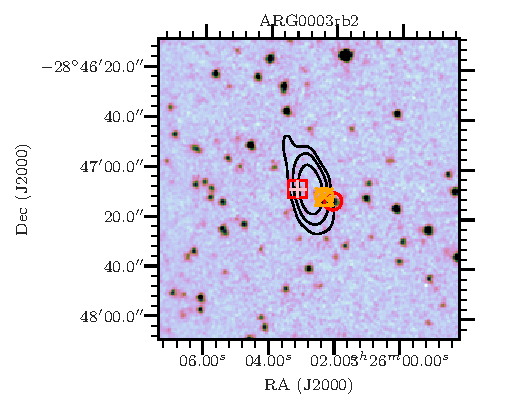
\includegraphics[width=\textwidth]{atlas-images/examples_all/example_sorted_2_0.pdf}
            \caption{One resolved component and resolved source.}
        \end{subfigure}
        \begin{subfigure}{0.45\textwidth}
            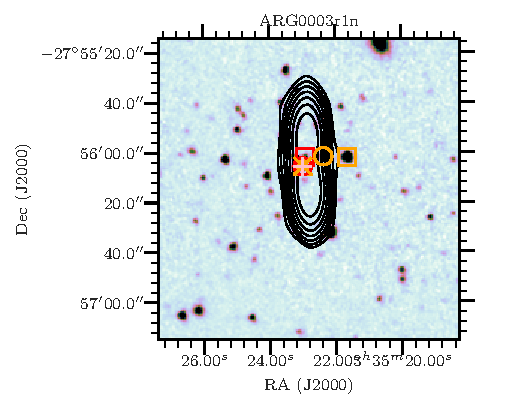
\includegraphics[width=\textwidth]{atlas-images/examples_all/example_sorted_3_454.pdf}
            \caption{Three resolved components comprising one resolved source.}
        \end{subfigure}
        \begin{subfigure}{0.45\textwidth}
            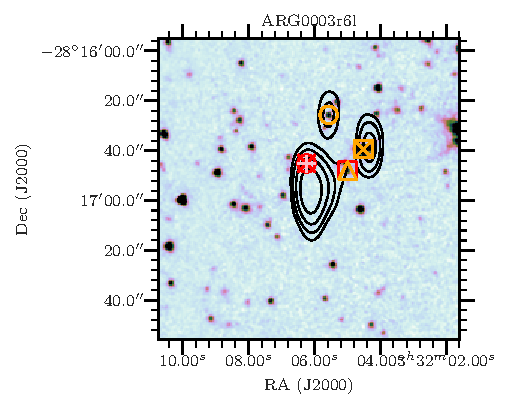
\includegraphics[width=\textwidth]{atlas-images/examples_all/example_sorted_4_264.pdf}
            \caption{Three resolved components comprising one resolved source.}
        \end{subfigure}
        \begin{subfigure}{0.45\textwidth}
            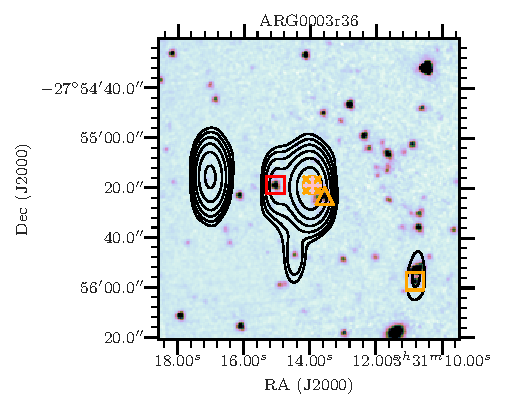
\includegraphics[width=\textwidth]{atlas-images/examples_all/example_sorted_5_207.pdf}
            \caption{Three resolved components comprising one resolved source.}
        \end{subfigure}
        \begin{subfigure}{0.9\textwidth}
            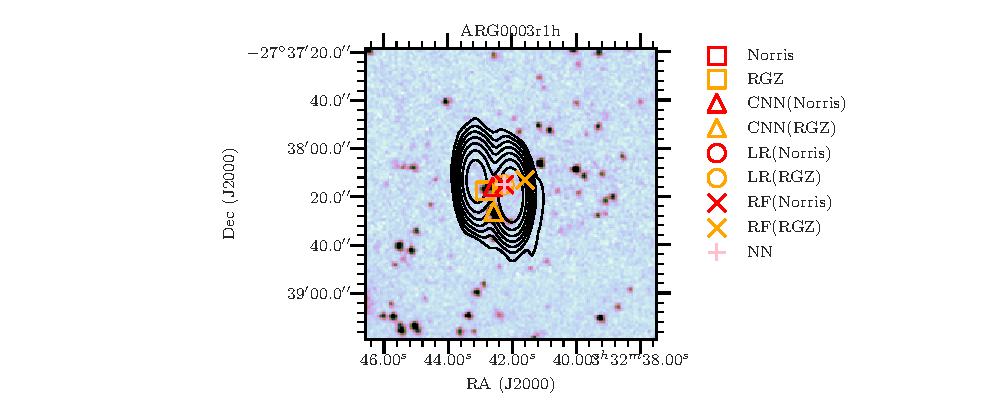
\includegraphics[width=\textwidth]{atlas-images/examples_all/example_sorted_0_306.pdf}
            \caption{Two compact components, each a compact source.}
        \end{subfigure}
        \caption[Examples of resolved sources with high disagreement between cross-identifiers.]{\label{fig:examples} Examples of resolved sources with high disagreement between cross-identifiers. The contours show ATLAS radio data and start at $4\sigma$, increasing geometrically by a factor of 2. The background image is the \unit{3.6}{\micro\meter} SWIRE image. Binary classifier model/training set combinations are denoted $C(S)$ where $C$ is the binary classifier model and $S$ is the training set. `LR' is logistic regression, `CNN' is convolutional neural networks, and `RF' is random forests. `Norris' refers to the expert labels and `RGZ' refers to the Radio Galaxy Zoo labels. The cross-identification made by nearest neighbours is shown by `NN'.}
    \end{figure}


  \section{Sankey diagrams}
  \label{sec:rlfs-sankey}

    This section presents Sankey diagrams showing the filtering of components and sources from the full FIRST sample in \autoref{cha:rlfs}, and was originally an appendix to \citet{alger21rlfs}. A Sankey diagram shows the order and number of objects removed from a sample. \autoref{fig:sankey-components} shows the filtering of components and \autoref{fig:sankey-sources} shows the filtering of sources. The component filters are `Bad FIRST' for components on the edge of FIRST with incomplete images, `Sidelobe' for components with high sidelobe probability, `Low score' for components with only low-scoring candidate hosts, `Faint' for components with less than 10 signal-to-noise according to the FIRST catalogue, and `Compact' for components that do not have extended radio emission according to \autoref{eq:rgz-criterion}. Sources were removed after each component filter if they no longer contained any components.

    \begin{figure}
        \centering
        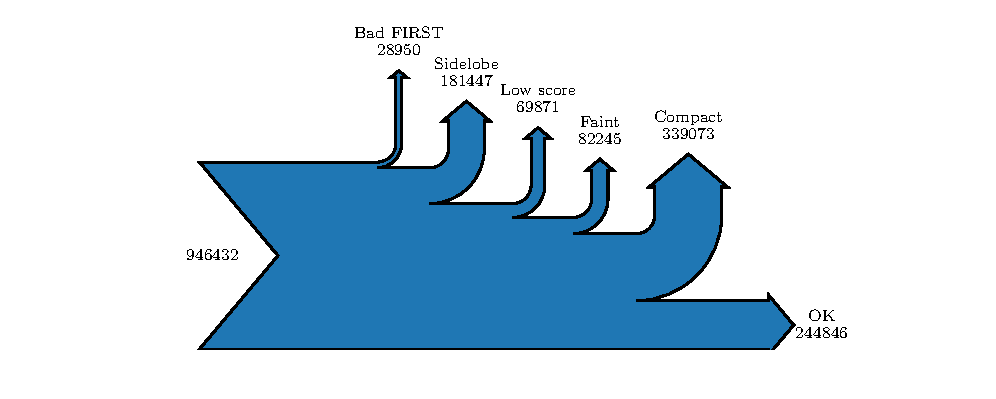
\includegraphics{rlf-images/sankey_components.pdf}
        \caption{\label{fig:sankey-components} Number of components removed from FIRST by each filter.}
    \end{figure}

    \begin{figure}
        \centering
        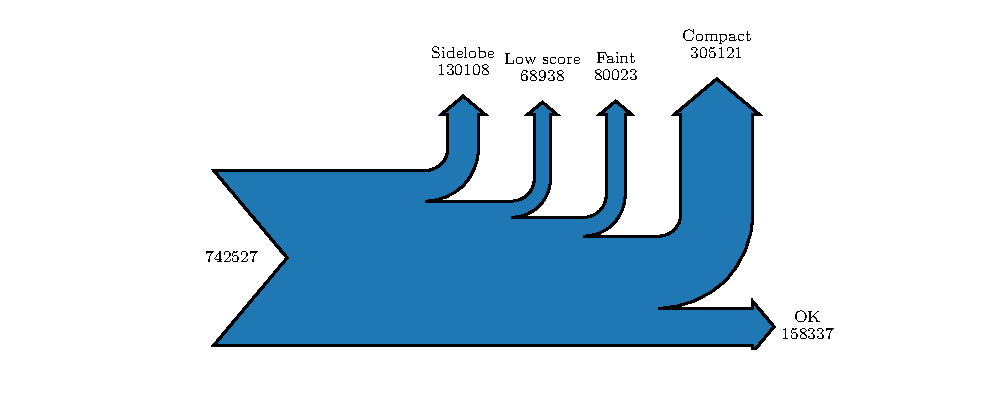
\includegraphics{rlf-images/sankey_sources.pdf}
        \caption{\label{fig:sankey-sources} Number of sources removed by each filter.}
    \end{figure}

\section{Radio luminosity function}
\label{sec:rlfs-rlf-desc}

  We computed the radio luminosity function following the $1/V_{\max}$ method
  \citep{schmidt1968vmax}. This appendix explains our implementation in \autoref{cha:rlfs} and was originally an appendix to \citet{alger21rlfs}. We performed the
  following steps:
  \begin{enumerate}
    \item Remove all radio sources that do not fit the selection criteria.
      This applies for both radio and infrared properties, so we choose a minimum radio flux density $f_{\min}$ and a maximum infrared magnitude
      $m_{\max}$, as well as redshift limits $z_{\mathrm{lower}}$ and $z_{\mathrm{upper}}$.
    \item For each source, compute the maximum redshift that the source could
      have been observed within the selection criteria. We find this redshift
      by first numerically solving \autoref{eq:luminosity} for $z$ with $L$ as
      the luminosity of each radio source and $f = f_{\min}$ to obtain the
      maximum redshift $z_\text{radio}$ at which the source could be observed
      in radio. We find the maximum redshift $z_{\text{ir}}$ that the host
      galaxy could be observed within the selection criteria by numerically
      solving \autoref{eq:ir-limits} for $z$, where $d(z)$ is the luminosity
      distance at a redshift $z$, $d$ is the luminosity distance of the host
      galaxy, and $m$ is the apparent magnitude of the host galaxy.
      \begin{equation}
        \label{eq:ir-limits}
        5 \log_{10}\left(\frac{d(z)}{d}\right) + m = m_{\max}
      \end{equation}
      The maximum redshift that the source could have been observed within the
      selection criteria is then $z_{\mathrm{max}} = \min(z_{\mathrm{ir}}, z_{\mathrm{radio}}, z_{\mathrm{upper}})$.
    \item For each source, compute the comoving volume $V_{\mathrm{max}}$ at
      redshift $z_{\mathrm{max}}$.
    \item The count for each luminosity bin is the sum over $1 / V_{\max}$ for
      each source in the bin. We divided these counts by the estimated completeness (\autoref{sec:rlfs-completeness}) to account for redshift incompleteness.
      We account for the fact FIRST does not cover the
      whole sky by multiplying by the total area of the sky divided by the area
      of our selection.
  \end{enumerate}

  After computing the luminosity function, we estimate the uncertainty in each bin using Poisson statistics, $\sqrt{N}$ for a bin count $N$.

  \section{Redshift completeness estimate}
  \label{sec:rlfs-completeness}

    \autoref{fig:completeness-wise} shows the estimated completeness of our RLF sample in \autoref{cha:rlfs} as a function of $W1$ and $W1-W2$. We followed the same method as \citet{pracy16rlf} for this estimation, averaging completeness over circles centred on each source. Each source is associated with a circle of radius equal to the distance to its 50th nearest neighbour in the $W1$ and $W1-W2$ plane. This appendix was originally part of \citet{alger21rlfs}.

    \begin{figure}
        \centering
        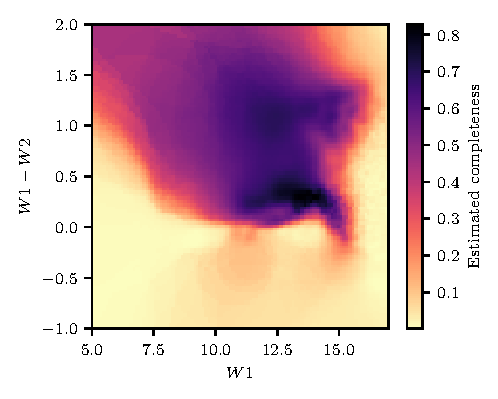
\includegraphics{rlf-images/completeness_wise.pdf}
        \caption{\label{fig:completeness-wise} Estimated completeness as a function of mid-infrared colour and magnitude.}
    \end{figure}

  \section{Giant radio galaxies}
  \label{sec:rlfs-giants}

    \begin{table*}
      \caption[Giant radio galaxies found in RGZ-Ex.]{\label{tab:grg} Giant radio galaxies found in RGZ-Ex. `LLS' is the projected linear size of the source as measured by the maximum angular distance between radio components. The RA/Dec are the coordinates of the host galaxy. s/p indicates spectroscopic/photometric redshift. ${}^L$Existing in literature. ${}^R$Also found by RGZ citizen scientists. ${}^\dagger$Misidentified SDSS host, manually corrected to obtain redshift.}
      \centering
      \begin{footnotesize}\begin{tabular}{c|ccccc}
  \hline\hline
  All\emph{WISE} host (WISEA) & RA (J2000) & Dec (J2000) & $z$ & LLS (Mpc) &\\
  \hline
    J004210.18-080011.3 & 10.54 & -8.00 & $0.65 \pm 0.14$ & 1.6 & p\\ % 3051
    J021008.48+011839.6${}^L$ & 32.54 & 1.31 & $0.86524 \pm 0.0001$ & 1.2 & s\\ % 8420
    J075858.29+355643.6${}^R$ & 119.74 & 35.95 & $0.74748 \pm 0.00013$ & 1.0 & s\\ % 19661
    J080831.68+473523.9${}^R$ & 122.13 & 47.59 & $0.58854 \pm 0.00016$ & 1.1 & s\\ % 21331
    J083034.78+231124.6 & 127.64 & 23.19 & $0.94 \pm 0.13$ & 1.1 & p\\ % 25768
    J090604.03+011114.2 & 136.52 & 1.19 & $0.7975 \pm 0.0004$ & 1.6 & s\\ % 33696
    J093256.81+074212.2 & 143.24 & 7.70 & $1.0032 \pm 0.0003$ & 1.1 & s\\ % 39983
    J093526.80+051729.8${}^R$ & 143.86 & 5.29 & $0.84 \pm 0.04$ & 1.2 & p\\ % 40574
    J094238.72+114337.9 & 145.66 & 11.73 & $0.49 \pm 0.05$ & 1.2 & p\\ % 42294
    J094835.60+535946.4${}^R$ & 147.15 & 54.00 & $0.64 \pm 0.10$ & 1.2 & p\\ % 43609
    J095706.12+292439.2 & 149.28 & 29.41 & $0.71 \pm 0.12$ & 1.5 & p\\ % 45638
    J102335.25+433208.0 & 155.90 & 43.54 & $0.75 \pm 0.09$ & 1.5 & p\\ % 51758
    J102933.99+210345.8${}^R$ & 157.39 & 21.06 & $0.82407 \pm 0.00008$ & 1.1 & s\\ % 53159
    J103043.98+355451.2${}^R$ & 157.68 & 35.91 & $0.64074 \pm 0.00008$ & 1.2 & s\\ % 53433
    J104449.92+234525.6${}^\dagger$ & 161.20 & 23.76 & $0.57712 \pm 0.00009$ & 1.6 & s\\ % 56652
    J110655.98+624759.8${}^R$ & 166.73 & 62.80 & $0.84379 \pm 0.00004$ & 1.1 & s\\ % 61882
    J112900.68+635543.2 & 172.25 & 63.93 & $0.71 \pm 0.06$ & 1.1 & p\\ % 67101
    J112948.20+243922.6 & 172.45 & 24.66 & $0.79 \pm 0.07$ & 1.1 & p\\ % 67288
    J114553.67-003304.7 & 176.47 & -0.55 & $2.0522 \pm 0.0006$ & 1.3 & s\\ % 71048
    J121111.26+534840.4 & 182.80 & 53.81 & $0.74 \pm 0.14$ & 1.1 & p\\ % 77051
    J121152.04+304232.4${}^R$ & 182.97 & 30.71 & $0.47102 \pm 0.00012$ & 1.3 & s\\ % 77229
    J121944.73+174121.3 & 184.94 & 17.69 & $1.5129 \pm 0.0009$ & 1.0 & s\\ % 79128
    J123735.89+544814.4${}^R$ & 189.40 & 54.80 & $1.0271 \pm 0.0006$ & 1.2 & s\\ % 83169
    J123819.16+113444.8 & 189.58 & 11.58 & $0.80 \pm 0.08$ & 1.2 & p\\ % 83310
    J123846.84-032857.5${}^\dagger$ & 189.70 & -3.48 & $0.67 \pm 0.07$ & 1.5 & p\\ % 83402
    J131625.00+272042.8 & 199.10 & 27.35 & $0.69092 \pm 0.00004$ & 1.0 & s\\ % 92344
    J133307.00+045048.6${}^R$ & 203.28 & 4.85 & $1.40534 \pm 0.00016$ & 1.1 & s\\ % 96197
    J141933.36+104706.4${}^R$ & 214.89 & 10.79 & $0.33973 \pm 0.00003$ & 1.0 & s\\ % 107030
    J142008.45+185422.7${}^R$ & 215.04 & 18.91 & $0.63 \pm 0.04$ & 1.4 & p\\ % 107197
    J145057.28+530007.7${}^L$ & 222.74 & 53.00 & $0.91662 \pm 0.00009$ & 1.3 & s\\ % 114664
    J150012.18+604941.3 & 225.05 & 60.83 & $1.6626 \pm 0.0007$ & 1.2 & s\\ % 116901
    J153547.13+432245.0${}^R$ & 233.95 & 43.38 & $0.63891 \pm 0.00007$ & 1.3 & s\\ % 125394
    J154631.18+194819.9 & 236.63 & 19.81 & $0.5917 \pm 0.0002$ & 1.4 & s\\ % 127907
    J160852.10+561110.2${}^R$ & 242.22 & 56.19 & $1.3196 \pm 0.0003$ & 1.3 & s\\ % 132855
    J162200.48+364044.0 & 245.50 & 36.68 & $1.9994 \pm 0.0002$ & 1.1 & s\\ % 135486
    J163004.35+103321.9${}^R$ & 247.52 & 10.56 & $0.85 \pm 0.09$ & 1.2 & p\\ % 136997
    J163125.75+200224.1${}^R$ & 247.86 & 20.04 & $0.62662 \pm 0.00013$ & 1.0 & s\\ % 137251
    J165055.46+394446.6 & 252.73 & 39.75 & $0.58829 \pm 0.00013$ & 1.1 & s\\ % 140491
    J232410.33+045309.6 & 351.04 & 4.89 & $0.76 \pm 0.06$ & 1.4 & p\\ % 156015
    J234440.02-003231.6 & 356.17 & -0.54 & $0.5014 \pm 0.0001$ & 1.0 & s\\ % 157352
      \hline\hline
      \end{tabular}\end{footnotesize}
    \end{table*}

    This appendix describes our search for giant radio galaxies in RGZ-Ex, and the results of this search. It was originally an appendix to \citet{alger21rlfs}. To identify radio sources we assumed that if any two components had the same host galaxy then they were part of the same source. This is a reasonable assumption if all host galaxies are correctly identified, which was not the case. This assumption therefore introduced spurious sources due to galaxies incorrectly identified as host galaxies: not all sources used in \autoref{cha:rlfs} are real sources, and in particular sources of large angular size are likely to be incorrect. Nevertheless RGZ-Ex provides a useful catalogue of \emph{candidate} radio sources, and visual follow-up can confirm whether sources of interest are real.

    H.A. and M.J.A. examined all 296 candidate sources in the RGZ-Ex catalogue with an estimated physical extent larger than 1~Mpc. Of these, 40 were real giant radio galaxies, which we show in \autoref{tab:grg}. We defined `giant radio galaxy' as a radio galaxy with emission extended to physical sizes $\geq 1.0$~Mpc. Other thresholds, such as $0.7$~Mpc, also exist in literature. The physical extents of the remaining 256 candidate sources were overestimated
mostly due to sidelobes/artefacts (103), incorrect source grouping (82), or incorrect SDSS matches (21). The citizen scientists who identified giants are: WizardHowl, DolorousEdd, antikodon, csunjoto, sisifolibre, JeanTate, JKD, PADV, and firejuggler. H.A., together with his summer students, had previously identified 29 of these giants.

    Note that this is a particularly challenging set: sources that are misidentified will often have unusually large estimated extents due to the inclusion of spurious components. The error rate in this set therefore does not reflect the rest of the catalogue.

\section{Visual verification results}
\label{sec:rlfs-verification-appendix}
  
  In \autoref{sec:rlfs-manual-validation} we described our visual verification of the BXID method from \autoref{cha:rlfs}. We list the radio components in the verification set in \autoref{tab:verification-set}. Each row of the table contains the FIRST component, its All\emph{WISE} host galaxy according to BXID, and whether the association is correct according to our visual verification. If an author was particularly unsure about an object, they were able to skip this object, and so are not accounted for in the verification for that object. Verification was weighted by the \citet{dawid79em} maximum likelihood model. This appendix was originally part of \citep{alger21rlfs}.

  \begin{table}
    \caption[Validation objects.]{\label{tab:verification-set} Validation objects. `Agree' is whether or not the authors of \citet{alger21rlfs} agreed with BXID associating the given FIRST object with the given All\emph{WISE} object.}
        \scriptsize\centering
      \begin{tabular}{ccc}
        \hline\hline
        FIRST & All\emph{WISE} & Agree\\\hline
        J000234.9-001421 & J000242.35-001320.5 & n\\
        J002841.1+141654 & J002840.37+141652.7 & y\\
        J003731.4+000156 & J003731.26+000146.7 & y\\
        J005407.5-011158 & J005407.61-011158.9 & y\\
        J011210.3+002203 & J011210.41+002201.9 & y\\
        J012342.4+015849 & J012342.24+015850.4 & y\\
        J013015.1+110653 & J013015.16+110653.4 & y\\
        J013107.7+070343 & J013102.02+070332.0 & y\\
        J014247.9-000039 & J014247.81-000040.3 & y\\
        J014250.0-000032 & J014247.81-000040.3 & n\\
        J020222.3+030138 & J020223.20+030150.4 & y\\
        J020333.8+000853 & J020336.94+000759.3 & y\\
        J021840.1-032311 & J021840.13-032306.0 & y\\
        J023022.0+010834 & J023022.11+010840.0 & y\\
        J024245.3-022535 & J024245.35-022534.6 & y\\
        J025901.0+005350 & J025901.50+005346.1 & y\\
        J033204.1-004757 & J033204.15-004757.1 & y\\
        J073033.2+390413 & J073033.21+390412.9 & y\\
        J073954.1+481810 & J073954.87+481759.5 & y\\
        J074504.9+331247 & J074504.81+331256.2 & y\\
        J074640.4+421709 & J074640.45+421709.1 & y\\
        J074707.9+171719 & J074708.35+171726.5 & y\\
        J075043.6+274838 & J075043.35+274844.8 & n\\
        J075050.3+331937 & J075051.25+331905.0 & y\\
        J075422.2+311253 & J075422.35+311252.5 & y\\
        J075637.0+212006 & J075636.65+212001.4 & y\\
        J082326.1+141438 & J082326.34+141435.9 & y\\
        J082422.5+351121 & J082422.65+351114.6 & y\\
        J082925.9+462618 & J082926.02+462618.5 & y\\
        J083512.4+175441 & J083512.45+175441.1 & y\\
        J084133.5+402035 & J084133.40+402042.8 & y\\
        J084238.4+405305 & J084238.38+405306.6 & n\\
        J084417.3+315845 & J084417.92+315845.9 & y\\
        J084728.5+360700 & J084728.24+360714.6 & y\\
        J084905.5+111448 & J084905.51+111447.8 & y\\
        J085236.8+262006 & J085236.11+262013.4 & y\\
        J085415.6+524930 & J085415.62+524936.7 & y\\
        J090623.2+300746 & J090622.87+300743.9 & y\\
        J091745.1+275049 & J091745.89+275103.8 & y\\
        J091752.0+431614 & J091752.14+431612.7 & y\\
        J092014.4+302907 & J092013.95+302859.3 & y\\
        J092140.5+540118 & J092140.24+540121.1 & y\\
        J092213.0+542157 & J092213.03+542157.2 & y\\
        J092406.9+562703 & J092406.47+562656.2 & y\\
        J092713.1+105841 & J092713.14+105839.8 & y\\
        J093108.6+613447 & J093108.63+613447.2 & y\\
        J093239.6+052308 & J093237.71+052240.7 & n\\
        J093627.8+103610 & J093627.87+103609.7 & y\\
        J093645.2+561435 & J093645.89+561434.2 & y\\
        J094006.8+482651 & J094006.92+482649.2 & y\\\hline\hline
  \end{tabular}
  \begin{tabular}{ccc}
        \hline\hline
        FIRST & All\emph{WISE} & Agree\\\hline
        J094009.5+600403 & J094011.55+600357.6 & n\\
        J094023.7+135123 & J094023.73+135125.2 & y\\
        J094324.5+435341 & J094324.61+435342.0 & y\\
        J094650.8+382015 & J094650.44+382010.9 & y\\
        J095011.8+455319 & J095011.82+455320.0 & y\\
        J095113.5+180211 & J095113.82+180204.2 & n\\
        J095242.4+222638 & J095242.45+222638.0 & y\\
        J095538.7+013546 & J095539.20+013546.1 & y\\
        J095609.9+363441 & J095609.30+363445.4 & y\\
        J095811.8+225056 & J095811.90+225055.5 & y\\
        J100019.2+263516 & J100018.84+263527.5 & y\\
        J101315.9+064520 & J101316.51+064519.0 & y\\
        J101455.2-004716 & J101455.30-004718.3 & y\\
        J102153.5+260429 & J102153.52+260429.6 & y\\
        J102354.7+390653 & J102354.88+390654.0 & y\\
        J102620.4+303600 & J102620.46+303550.4 & y\\
        J102710.4+460254 & J102714.81+460256.4 & n\\
        J102955.9+424906 & J102955.96+424906.7 & y\\
        J103503.9+102404 & J103503.92+102403.6 & y\\
        J103839.9+331200 & J103839.94+331201.1 & y\\
        J104030.5+211624 & J104031.09+211620.6 & n\\
        J104533.8+430025 & J104535.22+430020.8 & y\\
        J104907.5+322903 & J104907.91+322906.6 & y\\
        J105146.9+552257 & J105147.40+552308.4 & y\\
        J105257.5+105418 & J105257.53+105421.5 & y\\
        J105521.6+372641 & J105521.24+372652.4 & y\\
        J105758.8+321605 & J105758.84+321605.3 & y\\
        J110104.9+151618 & J110104.90+151618.2 & y\\
        J110353.2+352320 & J110353.37+352319.9 & y\\
        J110414.4+481345 & J110423.08+481311.0 & n\\
        J111057.7+220756 & J111057.18+220758.3 & y\\
        J111208.5+275207 & J111201.79+275053.8 & n\\
        J111225.2+233159 & J111225.30+233157.9 & y\\
        J111726.3+375336 & J111726.35+375337.0 & y\\
        J111746.1+261151 & J111746.18+261150.9 & y\\
        J111854.3+424708 & J111854.45+424652.8 & y\\
        J112124.4+640417 & J112125.02+640408.6 & y\\
        J112135.3+352330 & J112135.44+352324.9 & y\\
        J112550.9+200631 & J112558.75+200554.3 & y\\
        J112859.7+260923 & J112859.86+260911.3 & y\\
        J113201.1+442639 & J113201.23+442639.4 & y\\
        J113302.5+355408 & J113301.80+355415.3 & y\\
        J113712.7+263301 & J113711.86+263335.1 & y\\
        J113756.3+471314 & J113756.31+471314.1 & y\\
        J113906.6+230602 & J113906.68+230602.1 & y\\
        J114325.0+600721 & J114323.90+600737.1 & y\\
        J114759.7+370305 & J114759.22+370311.2 & y\\
        J114916.7+083022 & J114916.33+083040.5 & n\\
        J115010.9+063340 & J115010.93+063340.5 & y\\
        J115308.6+374851 & J115316.96+374850.0 & y\\\hline\hline
  \end{tabular}
\end{table}
\begin{table}
    \scriptsize\centering
  \begin{tabular}{ccc}
        \hline\hline
        FIRST & All\emph{WISE} & Agree\\\hline
        J115448.7+472222 & J115448.67+472223.7 & y\\
        J115603.7+584704 & J115603.48+584706.1 & y\\
        J115605.9+343230 & J115605.64+343229.4 & y\\
        J115653.0+572338 & J115645.38+572151.7 & y\\
        J120138.0+230922 & J120137.97+230922.2 & y\\
        J120752.8+533808 & J120752.85+533807.3 & y\\
        J120943.3-021934 & J120942.89-021943.0 & y\\
        J121045.6+190225 & J121045.68+190227.0 & y\\
        J121207.6+115412 & J121207.72+115413.8 & y\\
        J121211.3+485951 & J121211.86+485952.0 & y\\
        J121406.7+002634 & J121406.73+002635.0 & y\\
        J122518.0+350258 & J122517.85+350301.9 & y\\
        J122525.1+451530 & J122524.71+451508.5 & y\\
        J122640.9+430508 & J122640.82+430509.2 & y\\
        J123429.8+260107 & J123434.79+260134.3 & n\\
        J123633.1+100928 & J123633.12+100928.7 & y\\
        J124839.3+411522 & J124839.42+411522.3 & n\\
        J125129.2+551012 & J125128.76+551009.3 & y\\
        J130005.8+524801 & J130006.14+524803.0 & y\\
        J130132.1+511351 & J130132.32+511352.5 & y\\
        J131104.4+464936 & J131104.45+464934.0 & y\\
        J131452.2+252811 & J131446.81+252820.8 & n\\
        J132033.8+332639 & J132033.59+332639.0 & n\\
        J132257.5+191134 & J132257.53+191133.9 & y\\
        J132529.3+230734 & J132529.35+230733.8 & y\\
        J132546.8+052453 & J132546.86+052454.1 & y\\
        J132637.7+112110 & J132637.92+112108.8 & y\\
        J132831.8+104339 & J132831.88+104338.8 & y\\
        J132932.3+131839 & J132932.32+131839.6 & y\\
        J133022.8+311904 & J133022.83+311902.8 & y\\
        J133453.3+405653 & J133454.13+405650.6 & y\\
        J133741.1+124302 & J133741.13+124303.1 & y\\
        J133823.6+103337 & J133823.67+103341.9 & y\\
        J134651.2+415154 & J134651.06+415156.1 & y\\
        J134704.3+110622 & J134704.35+110622.7 & y\\
        J134752.7+555046 & J134752.71+555048.6 & y\\
        J134831.7+164325 & J134831.57+164328.2 & y\\
        J134949.8+385539 & J134949.93+385542.8 & y\\
        J135106.5+074534 & J135106.50+074534.2 & y\\
        J135107.7+615502 & J135107.75+615502.1 & y\\
        J135658.5+134028 & J135659.15+134017.0 & y\\
        J135833.9+180021 & J135834.03+180020.4 & y\\
        J140630.7+554017 & J140629.32+554009.9 & y\\
        J140804.2+503019 & J140804.10+503021.1 & y\\
        J141226.7+454125 & J141226.54+454125.5 & y\\
        J141245.0+495213 & J141243.84+495206.4 & y\\
        J141317.4+325306 & J141317.50+325306.8 & y\\
        J141723.8+543639 & J141724.33+543629.5 & y\\
        J141938.8+312146 & J141940.16+312138.8 & y\\
        J142515.3+175526 & J142513.89+175525.7 & y\\\hline\hline
  \end{tabular}
  \begin{tabular}{ccc}
        \hline\hline
        FIRST & All\emph{WISE} & Agree\\\hline
        J142829.5+070836 & J142829.60+070836.3 & y\\
        J143411.0+170036 & J143411.18+170035.7 & y\\
        J143624.0-001057 & J143623.89-001100.8 & y\\
        J143742.6+104412 & J143742.69+104412.8 & y\\
        J143840.8+475355 & J143841.08+475356.1 & y\\
        J143909.1+430847 & J143909.08+430847.8 & y\\
        J144135.8+102246 & J144135.91+102245.1 & y\\
        J144333.6+275229 & J144333.02+275250.2 & y\\
        J145012.3+471739 & J145012.33+471738.7 & y\\
        J145103.7+452459 & J145102.66+452520.5 & n\\
        J145401.6+141009 & J145401.70+141009.6 & y\\
        J150158.7+191413 & J150158.87+191405.3 & y\\
        J150743.9+352720 & J150743.62+352724.1 & y\\
        J151141.6-003209 & J151142.01-003213.0 & y\\
        J151315.5+403107 & J151315.56+403107.7 & y\\
        J151518.7+230256 & J151518.67+230257.3 & y\\
        J151703.6+105947 & J151703.68+105947.6 & y\\
        J151736.8+610856 & J151736.83+610857.7 & y\\
        J152121.6+281635 & J152120.68+281626.2 & y\\
        J152714.8+310425 & J152714.88+310424.7 & y\\
        J153428.9+272134 & J153429.68+272120.8 & y\\
        J154245.3+100919 & J154245.71+100917.8 & y\\
        J154901.6+103159 & J154901.40+103152.6 & y\\
        J154925.2+395316 & J154926.17+395303.7 & y\\
        J155206.3-005348 & J155206.58-005339.3 & y\\
        J155457.3+344637 & J155458.45+344644.7 & y\\
        J155743.5+272752 & J155743.52+272752.8 & y\\
        J160130.0+083848 & J160130.07+083850.7 & y\\
        J160534.8+441220 & J160535.55+441221.5 & y\\
        J160859.2+400135 & J160901.32+400230.7 & n\\
        J161545.4+231617 & J161545.14+231617.2 & y\\
        J161930.4+085533 & J161930.51+085532.6 & y\\
        J162228.0+264743 & J162228.70+264736.7 & y\\
        J162750.4+473624 & J162750.55+473623.5 & y\\
        J162904.2+470852 & J162904.34+470853.0 & y\\
        J163038.7+214740 & J163037.43+214748.9 & n\\
        J163323.6+424051 & J163323.61+424051.9 & y\\
        J163327.5+242426 & J163327.87+242427.4 & y\\
        J163533.8+454557 & J163534.00+454554.3 & y\\
        J164211.2+512029 & J164211.27+512029.3 & y\\
        J165549.1+375923 & J165549.01+375923.6 & y\\
        J165620.0+363402 & J165619.89+363403.9 & y\\
        J165700.5+474820 & J165659.58+474809.0 & y\\
        J171406.2+292712 & J171404.16+292704.0 & n\\
        J172126.4+374446 & J172126.46+374446.6 & y\\
        J222627.7-005010 & J222627.77-005010.8 & y\\
        J223636.4-013827 & J223636.48-013827.2 & y\\
        J225619.0+143257 & J225621.96+143351.4 & y\\
        J232410.1+001315 & J232410.15+001314.5 & y\\
        J234727.9-000919 & J234727.65-000912.9 & y\\\hline\hline
  \end{tabular}
\end{table}

\section{2-Wasserstein begets Faraday moments}
  \label{sec:faraday-w2-to-faraday-moments}
    Minimising the 2-Wasserstein distance between a model FDF and the simple manifold gives the second Faraday moment of that FDF. This appendix demonstrates that fact, and was originally part of \citet{alger2021interpretable}. Let $\tilde F$ be the sum-normalised model FDF and let $\tilde S$ be the sum-normalised simple model FDF:
    \begin{align}
      \tilde F(\phi) &= \frac{A_0 \delta(\phi - \phi_0) + A_1 \delta(\phi - \phi_1)}{A_0 + A_1}\\
      \tilde S(\phi; \phi_w) &= \delta(\phi - \phi_w).
    \end{align}
    The $W_2$ distance, usually defined on probability distributions, can be extended to one-dimensional complex functions $A$ and $B$ by normalising them:
      \begin{align}
        \label{eq:faraday-w2}
        D_{W_2}\infdivx{A}{B}^2 &= \inf_{\gamma \in \Gamma(A, B)} \iint_{\phi_{\min}}^{\phi_{\max}} |x - y|^2\ \mathrm{d}\gamma(x, y) \\
        \label{eq:faraday-normalised}
        \tilde A(\phi) &= \frac{|A(\phi)|}{\int_{\phi_{\min}}^{\phi_{\max}} |A(\theta)|\ \mathrm{d}\theta}\\
        \tilde B(\phi) &= \frac{|B(\phi)|}{\int_{\phi_{\min}}^{\phi_{\max}} |B(\theta)|\ \mathrm{d}\theta}
      \end{align}
      where $\Gamma(A, B)$ is the set of couplings of $A$ and $B$, i.e. the set of joint probability distributions that marginalise to $A$ and $B$; and $\inf_{\gamma \in \Gamma(A, B)}$ is the infimum over $\Gamma(A, B)$. This can be interpreted as the minimum cost to `move' one probability distribution to the other, where the cost of moving one unit of probability mass is the squared distance it is moved.

    The set of couplings $\Gamma(\tilde F, \tilde S)$ is the set of all joint probability distributions $\gamma$ such that
    \begin{align}
      \int_{\phi_{\min}}^{\phi_{\max}} \gamma(\phi, \varphi)\ \mathrm{d}\phi &= \tilde S(\varphi; \phi_w),\\
      \int_{\phi_{\min}}^{\phi_{\max}} \gamma(\phi, \varphi)\ \mathrm{d}\varphi &= \tilde F(\phi).
    \end{align}
    The coupling that minimises the integral in \autoref{eq:faraday-w2} will be the optimal transport plan between $\tilde F$ and $\tilde S$. Since $\tilde F$ and $\tilde S$ are defined in terms of delta functions, the optimal transport problem reduces to a discrete optimal transport problem and the optimal transport plan is:
    \begin{equation}
      \gamma(\phi, \varphi) = \frac{A_0 \delta(\phi - \phi_0) + A_1 \delta(\phi - \phi_1)}{A_0 + A_1} \delta(\varphi - \phi_w).
    \end{equation}
    In other words, to move the probability mass of $\tilde S$ to $\tilde F$, a fraction $A_0/(A_0 + A_1)$ is moved from $\phi_w$ to $\phi_0$ and the complementary fraction $A_1/(A_0 + A_1)$ is moved from $\phi_w$ to $\phi_1$. Then:
    \begin{align}
      D_{W_2}\infdivx{\tilde F}{\tilde S}^2 &= \iint_{\phi_{\min}}^{\phi_{\max}} |\phi - \varphi|^2\ \mathrm{d}\gamma(\phi, \varphi)\\
        &= \frac{A_0 (\phi_0 - \phi_w)^2 + A_1 (\phi_1 - \phi_w)^2}{A_0 + A_1}.
    \end{align}
    To obtain the $W_2$ distance to the simple manifold, we need to minimise this over $\phi_w$. Differentiate with respect to $\phi_w$ and set equal to zero to find
    \begin{equation}
      \phi_w = \frac{A_0 \phi_0 + A_1 \phi_1}{A_0 + A_1}.
    \end{equation}
    Substituting this back in, we find
    \begin{align}
      \varsigma_{W_2}(F)^2 &= \frac{A_0 A_1}{A_0 + A_1}(\phi_0 - \phi_1)^2
    \end{align}
    which is the Faraday moment.

\section{Euclidean distance in the no-RMSF case}
\label{sec:faraday-euclidean-calculation}

  In this appendix, originally from \citet{alger2021interpretable}, we calculate the minimised Euclidean distance evaluated on a model FDF (\autoref{eq:faraday-true-fdf}). Let $\tilde F$ be the sum-normalised model FDF and let $\tilde S$ be the normalised simple model FDF:
  \begin{align}
    \tilde F(\phi) &= \frac{A_0 \delta(\phi - \phi_0) + A_1 \delta(\phi - \phi_1)}{A_0 + A_1}\\
    \tilde S(\phi; \phi_e) &= \delta(\phi - \phi_e).
  \end{align}

  The Euclidean distance between $\tilde F$ and $\tilde S$ is then
  \begin{align}
    &D_E\infdivx{\tilde F(\phi)}{\tilde S(\phi; \phi_e)}^2\\
    &= \int_{\phi_{\min}}^{\phi_{\max}} \left|\tilde F(\phi) - \delta(\phi - \phi_e) \right|^2\ \mathrm{d}\phi.
  \end{align}

  Assume $\phi_0 \neq \phi_1$ (otherwise, $D_E$ will always be either $0$ or $2$). If $\phi_e = \phi_0$, then
  \begin{align}
    &D_E\infdivx{\tilde F(\phi)}{\tilde S(\phi; \phi_e)}^2\\
      &= \frac{1}{(A_0 + A_1)^2} \int_{\phi_{\min}}^{\phi_{\max}} A_1^2 \left|\delta(\phi - \phi_1) - \delta(\phi - \phi_0) \right|^2\ \mathrm{d}\phi\\
      &= \frac{2 A_1^2}{(A_0 + A_1)^2}
  \end{align}
  and similarly for $\phi_e = \phi_1$. If $\phi_e \neq \phi_0$ and $\phi_e \neq \phi_1$, then
  \begin{equation}
    D_E\infdivx{\tilde F(\phi)}{\tilde S(\phi; \phi_e)}^2 = \frac{A_0^2 + A_1^2 + 1}{(A_0 + A_1)^2}.
  \end{equation}
  The minimised Euclidean distance when $\phi_0 \neq \phi_1$ is therefore
  \begin{align}
      D_E(F) &= \min_{\phi_e \in \mathbb{R}} D_E\infdivx{F(\phi)}{F_{\mathrm{simple}}(\phi; \phi_e)}\\
          &= \sqrt{2} \frac{\min(A_0, A_1)}{A_0 + A_1}.
  \end{align}
  If $\phi_0 = \phi_1$, then the minimised Euclidean distance is 0.

\section{Hyperparameters for LR and XGB}
\label{sec:faraday-hyperparameters}

  This section contains tables of the hyperparameters that we used for our classifiers in \autoref{cha:faraday} and was originally an appendix to \citet{alger2021interpretable}. \autoref{tab:faraday-hyperparameters-xgb} and \autoref{tab:faraday-hyperparameters-lr} tabulate the hyperparameters for XGB and LR respectively for the `ATCA' dataset. \autoref{tab:faraday-hyperparameters-xgb-askap12} and \autoref{tab:faraday-hyperparameters-lr-askap12} tabulate the hyperparameters for XGB and LR respectively for the `ASKAP' dataset.

  \begin{table}[htbp]
    \caption{\label{tab:faraday-hyperparameters-xgb} XGB hyperparameters for the `ATCA' dataset.}
    \centering
    \begin{tabular}{ll}
      \hline\hline
      Parameter & Value\\\hline
      colsample\textunderscore{}bytree & 0.912\\
      gamma & 0.532\\
      learning\textunderscore{}rate & 0.1\\
      max\textunderscore{}depth & 7\\
      min\textunderscore{}child\textunderscore{}weight & 2\\
      scale\textunderscore{}pos\textunderscore{}weight & 1\\
      subsample & 0.557\\
      n\textunderscore{}estimators & 135\\
      reg\textunderscore{}alpha & 0.968\\
      reg\textunderscore{}lambda & 1.420\\
      \hline\hline
    \end{tabular}
  \end{table}

  \begin{table}[htbp]
    \caption{\label{tab:faraday-hyperparameters-lr} LR hyperparameters for the `ATCA' dataset.}
    \centering
    \begin{tabular}{ll}
      \hline\hline
      Parameter & Value\\\hline
      penalty & L1\\
      C & 1.668\\
      \hline\hline
    \end{tabular}
  \end{table}

  \begin{table}[htbp]
    \caption{\label{tab:faraday-hyperparameters-xgb-askap12} XGB hyperparameters for the `ASKAP' dataset.}
    \centering
    \begin{tabular}{ll}
      \hline\hline
      Parameter & Value\\\hline
      colsample\textunderscore{}bytree & 0.865\\
      gamma & 0.256\\
      learning\textunderscore{}rate & 0.1\\
      max\textunderscore{}depth & 6\\
      min\textunderscore{}child\textunderscore{}weight & 1\\
      scale\textunderscore{}pos\textunderscore{}weight & 1\\
      subsample & 0.819\\
      n\textunderscore{}estimators & 108\\
      reg\textunderscore{}alpha & 0.049\\
      reg\textunderscore{}lambda & 0.454\\
      \hline\hline
    \end{tabular}
  \end{table}

  \begin{table}[htbp]
    \caption{\label{tab:faraday-hyperparameters-lr-askap12} LR hyperparameters for the `ASKAP' dataset.}
    \centering
    \begin{tabular}{ll}
      \hline\hline
      Parameter & Value\\\hline
      penalty & L2\\
      C & 0.464\\
      \hline\hline
    \end{tabular}
  \end{table}

\section{Predictions on real data}
\label{sec:faraday-real-data-fig}

  This appendix, originally part of \citet{alger2021interpretable}, contains \autoref{fig:faraday-all-observed-fdfs-lr} and \autoref{fig:faraday-all-observed-fdfs-xgb}. These show the predicted probability of being Faraday complex for all real data used in \autoref{cha:faraday}, drawn from \citet{livingston21faraday} and \citet{osullivan_broad-band_2017}.

  \begin{figure*}
    \centering
    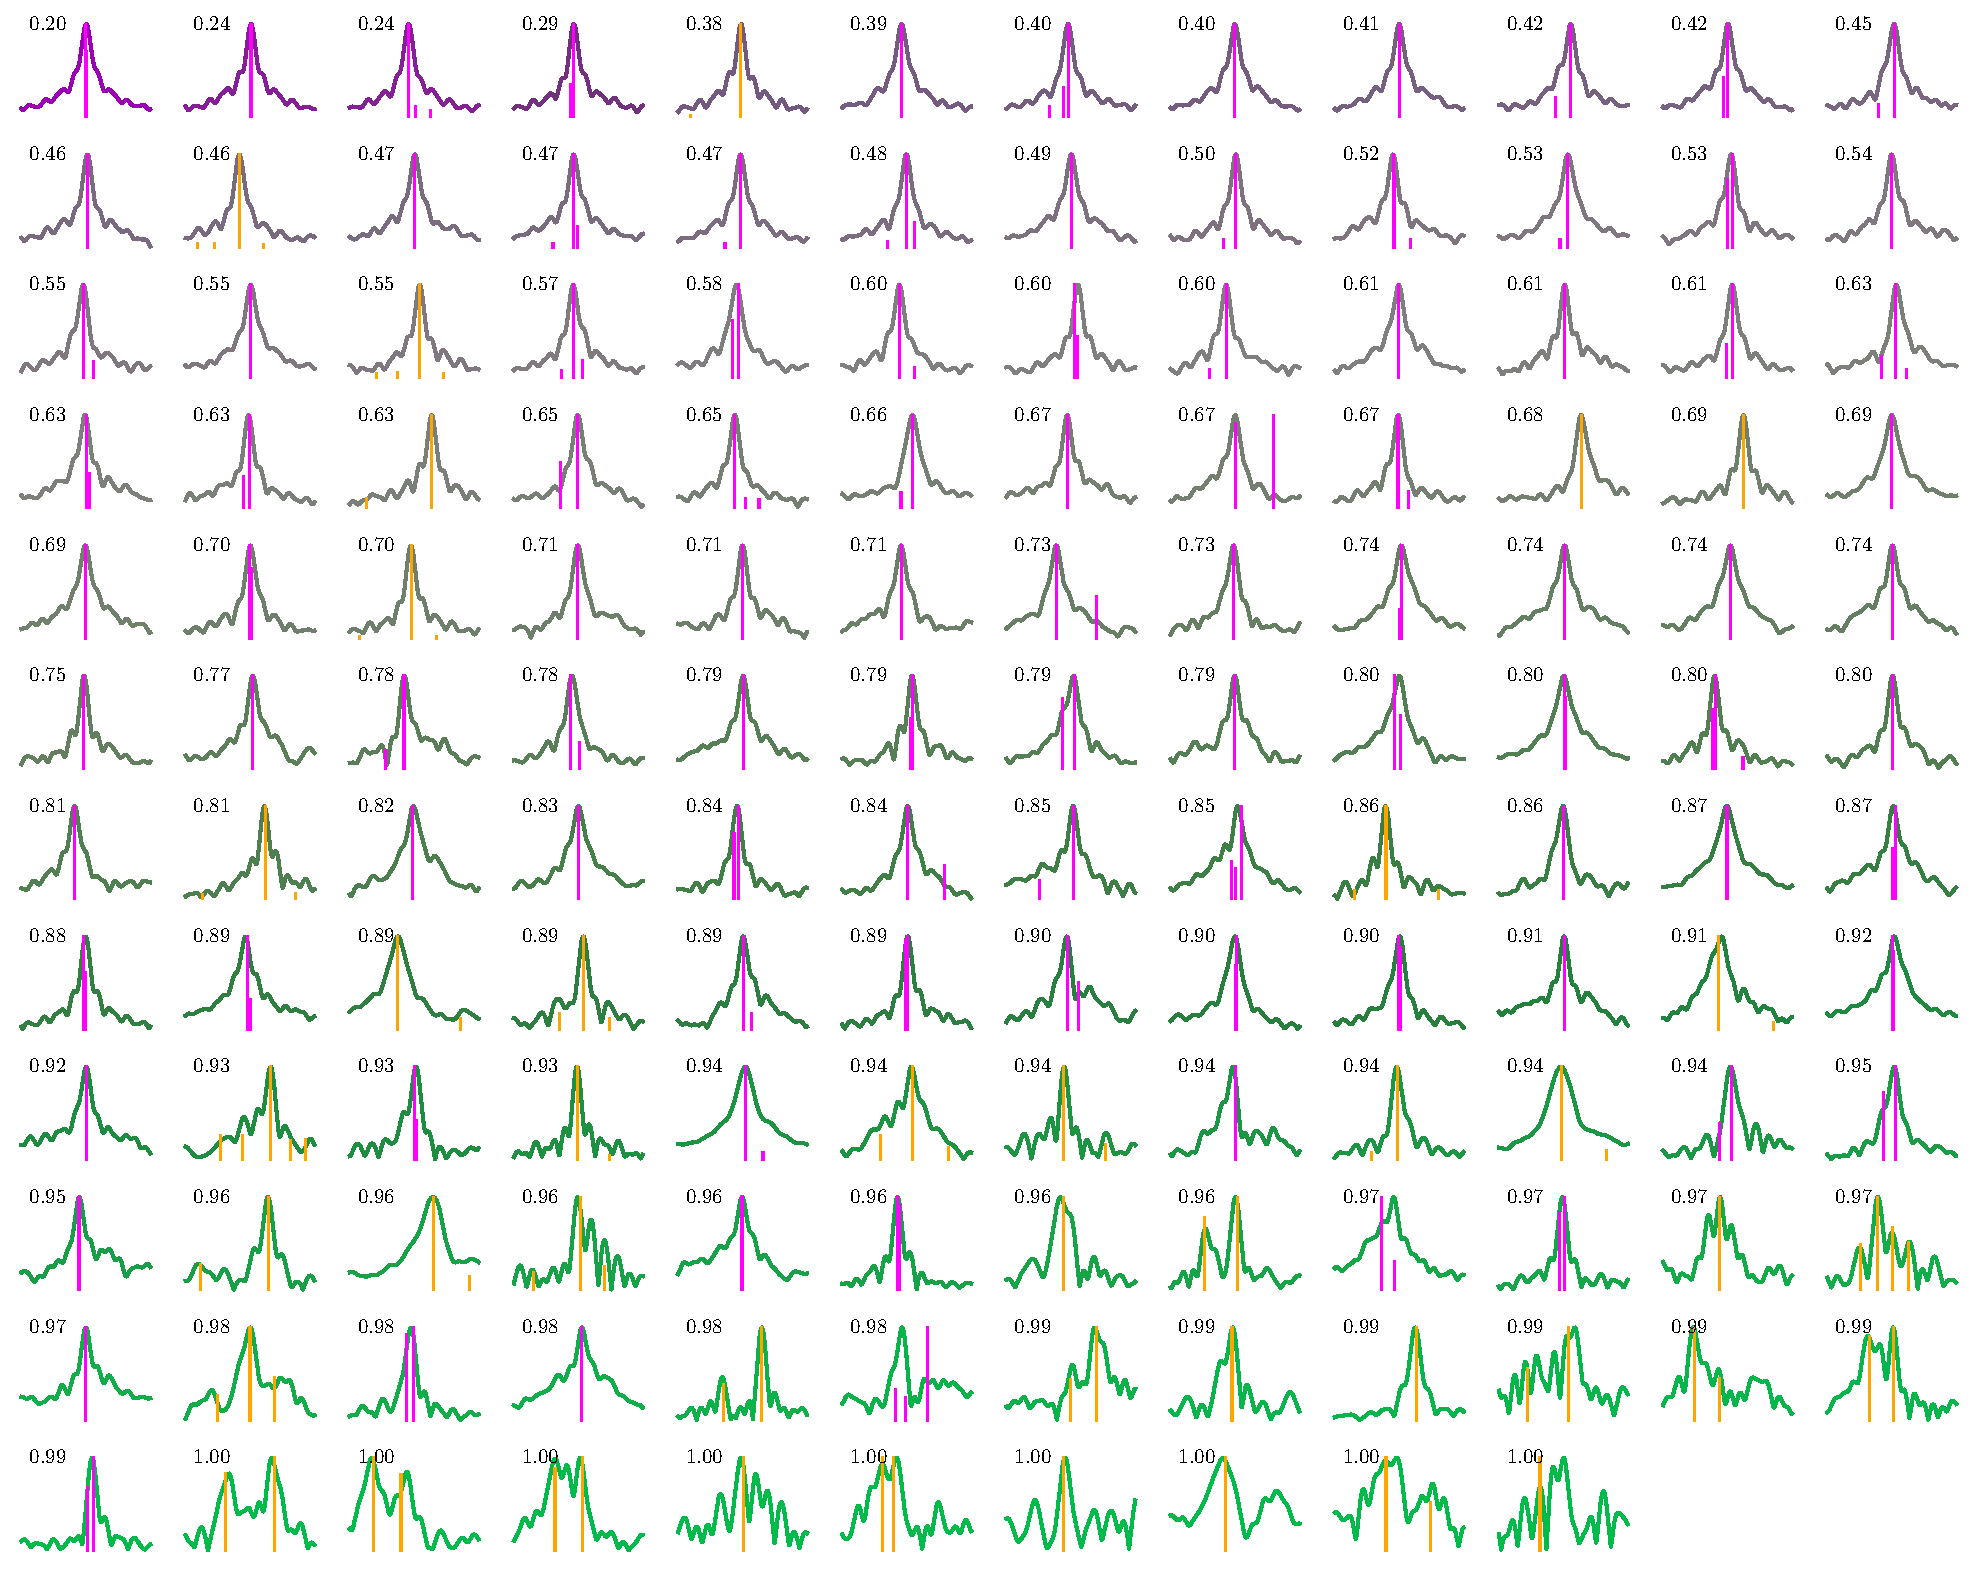
\includegraphics[width=\linewidth]{faraday-images/both_spectra_lr.pdf}
    \caption[The 142 observed FDFs ordered by LR-estimated probability of being Faraday complex.]{The 142 observed FDFs ordered by LR-estimated probability of being Faraday complex. Livingston-identified components are shown in orange while O'Sullivan-identified components are shown in magenta. Simpler FDFs (as deemed by the classifier) are shown in purple while more complex FDFs are shown in green, and the numbers overlaid indicate the LR estimate. A lower number indicates a lower probability that the corresponding source is complex, i.e. lower numbers correspond to simpler spectra.}
    \label{fig:faraday-all-observed-fdfs-lr}
  \end{figure*}

  \begin{figure*}
    \centering
    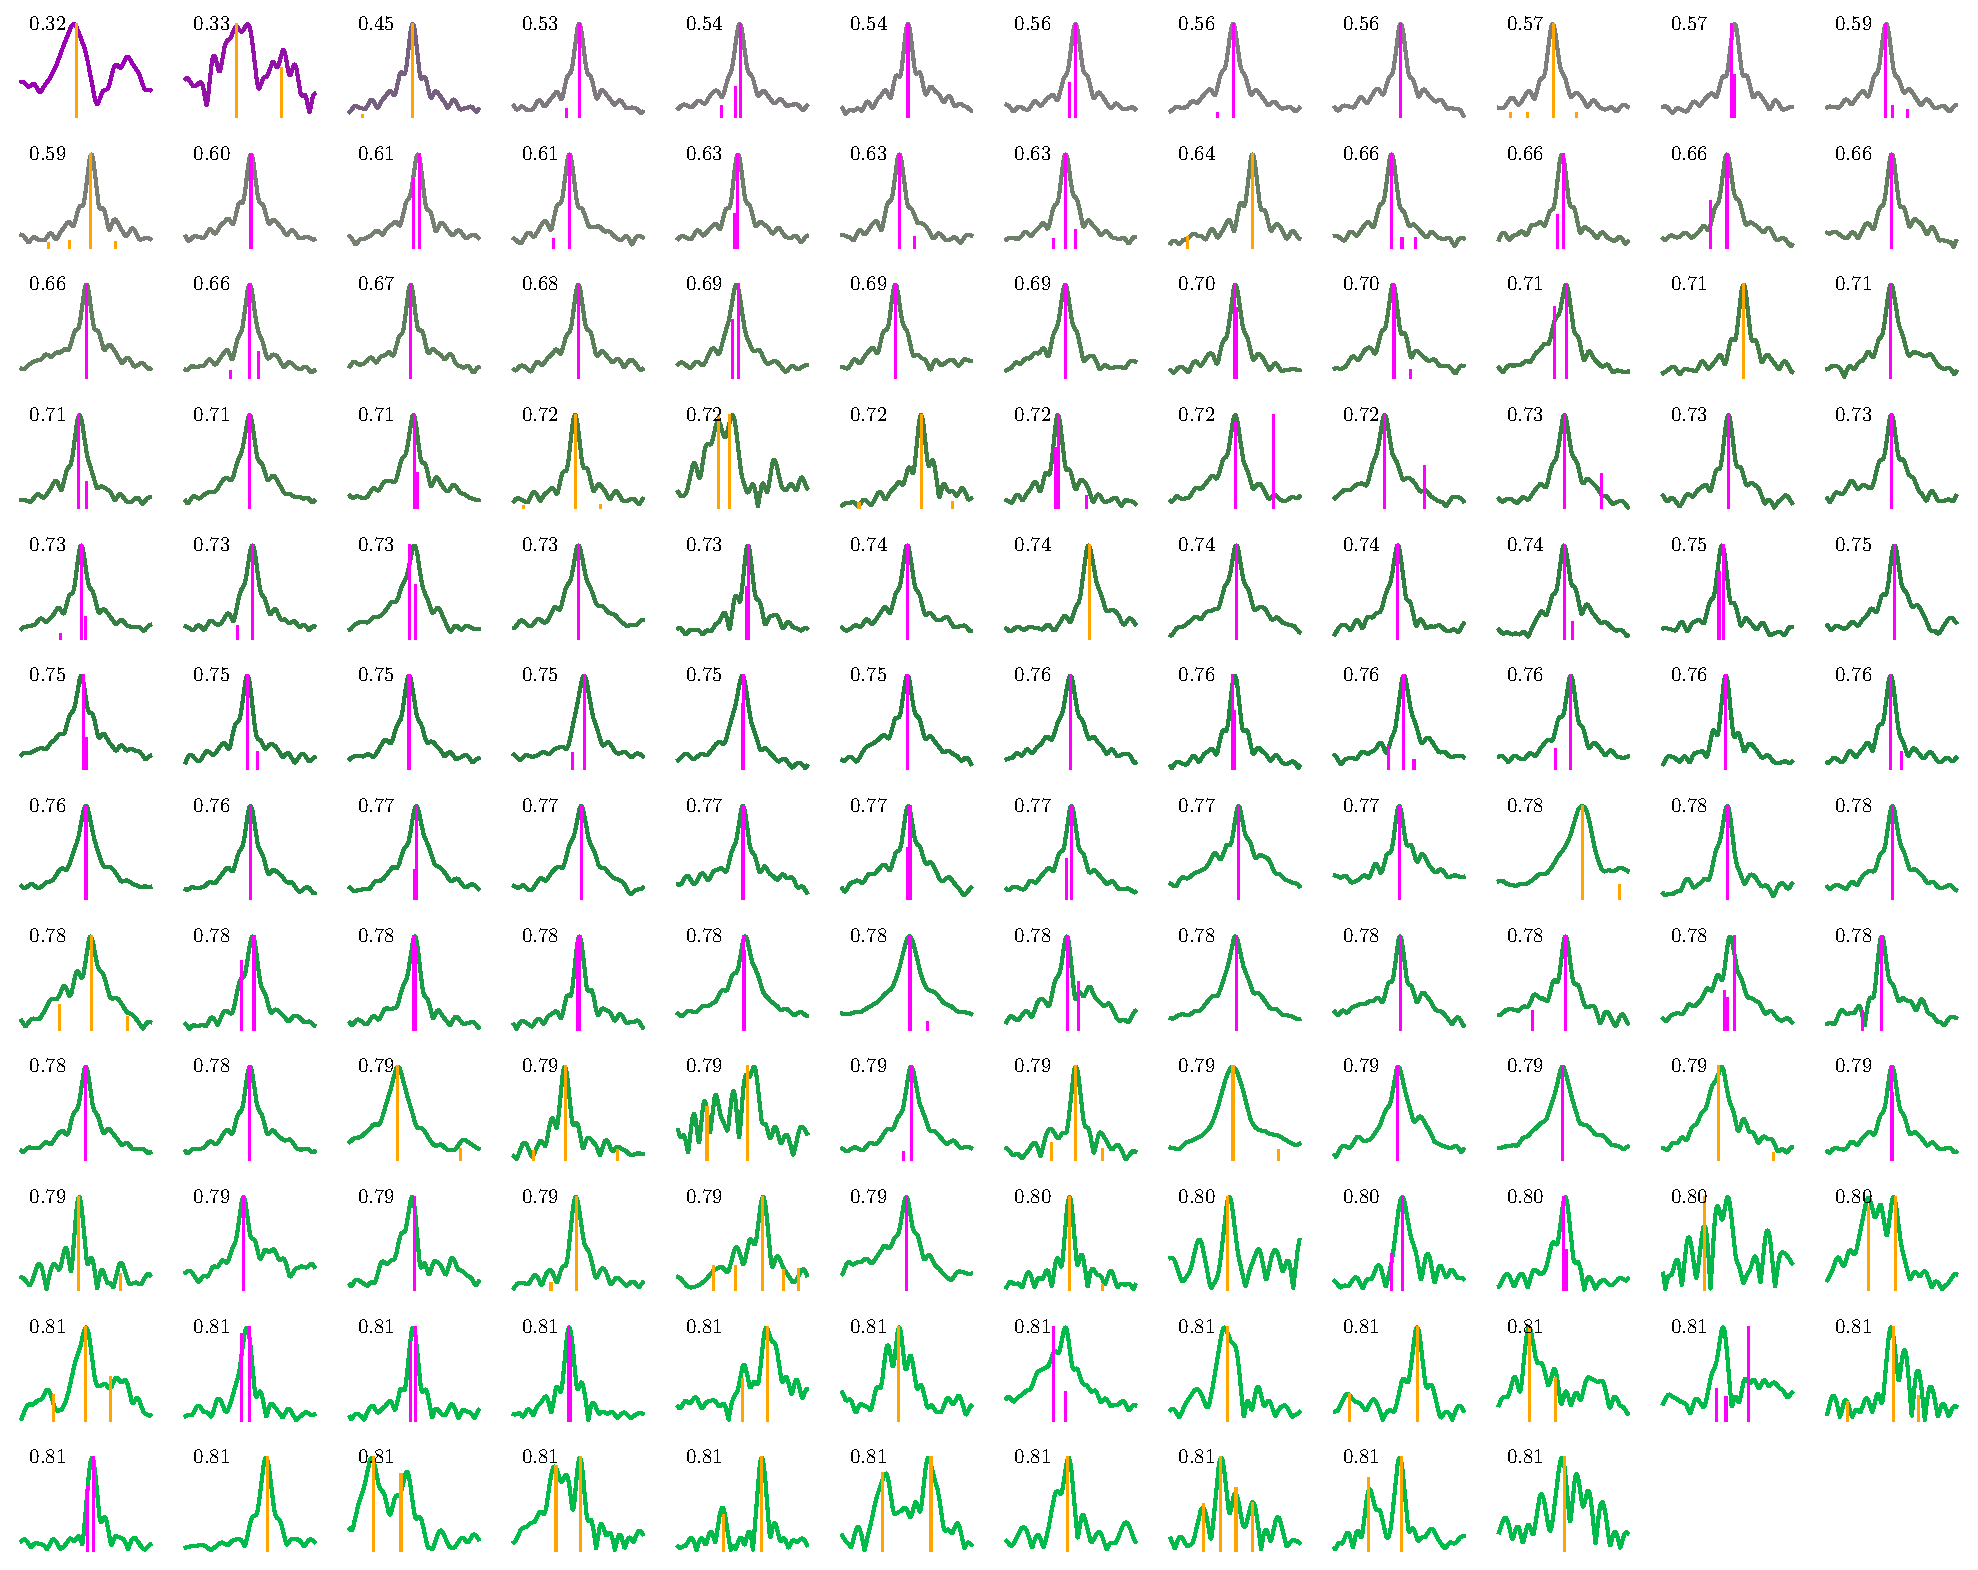
\includegraphics[width=\linewidth]{faraday-images/both_spectra_xgb.pdf}
    \caption[The 142 observed FDFs ordered by XGB-estimated probability of being Faraday complex.]{The 142 observed FDFs ordered by XGB-estimated probability of being Faraday complex. Livingston-identified components are shown in orange while O'Sullivan-identified components are shown in magenta. Simpler FDFs (as deemed by the classifier) are shown in purple while more complex FDFs are shown in green, and the numbers overlaid indicate the XGB estimate. A lower number indicates a lower probability that the corresponding source is complex, i.e. lower numbers correspond to simpler spectra.}
    \label{fig:faraday-all-observed-fdfs-xgb}
  \end{figure*}

\section{Simulating observed FDFs}
\label{sec:faraday-simulating}

  This appendix was originally part of \citet{alger2021interpretable} and describes how we simulated FDFs in \autoref{cha:faraday}. We simulated FDFs by approximating them by arrays of complex numbers. An FDF $F$ is approximated on the domain $[-\phi_{\max}, \phi_{\max}]$ by a vector $\vec F \in \mathbb R^d$:
    \begin{equation}
      \label{eq:faraday-vec-f}
      \vec F_j = \sum_{k = 0}^1 A_k \delta(-\phi_{\max} + j \delta \phi - \phi_k)
    \end{equation}
    where $\delta\phi = (\phi_{\max} - \phi_{\min}) / d$ and $d$ is the number of Faraday depth samples in the FDF.
    $\vec F$ is sampled by uniformly sampling its parameters:
    \begin{align}
      \label{eq:faraday-model-distributions}
      \phi_k &\in [\phi_{\min}, \phi_{\min} + \delta\phi, \dots, \phi_{\max}]\\
      A_k &\sim \mathcal U(0, 1).
    \end{align}
    We then generate a vector polarisation spectrum $\vec P \in \mathbb R^m$ from $\vec F$ using a \autoref{eq:faraday-discrete-f-to-p}:
    \begin{equation}
      \label{eq:faraday-discrete-f-to-p}
      \vec P_\ell = \sum_{j = 0}^{j} F_j e^{2i(\phi_{\min} + j\delta_\phi)\lambda^2_\ell}\ \mathrm{d}\phi.
    \end{equation}
    $\lambda^2_\ell$ is the discretised value of $\lambda^2$ at the $\ell$th index of $\vec P$. This requires a set of $\lambda^2$ values, which depends on the dataset being simulated. These values can be treated as the channel wavelengths at which the polarisation spectrum was observed. We then add Gaussian noise with variance $\sigma^2$ to each element of $\vec P$ to obtain a discretised noisy observation $\hat{\vec{P}}$. Finally, we perform RM synthesis using the Canadian Initiative for Radio Astronomy Data Analysis \texttt{RM} package\footnote{\url{https://github.com/CIRADA-Tools/RM}}, which is a \texttt{Python} module that implements a discrete version of RM synthesis:
    \begin{equation}
      \label{eq:faraday-discrete-rm-synthesis}
      \hat{\vec{F}}_j = m^{-1} \sum_{\ell = 1}^m \vec{\hat P}_\ell e^{-2i(\phi_{\min} + j\delta_\phi)\lambda^2_\ell}.
    \end{equation}